\documentclass[14pt, table]{extarticle}
\usepackage{amsfonts}
\usepackage{amsmath}
\usepackage[utf8]{inputenc}
\usepackage[a4paper, total={7in, 10.5in}]{geometry}
\usepackage[table]{xcolor}
\usepackage{tgbonum}
\usepackage{float}
\usepackage{graphicx}
\graphicspath{ {./images/} }
\DeclareGraphicsExtensions{.png,.jpg}
\usepackage{caption}
\usepackage{tikz}
\usepackage{circuitikz}
\usepackage[T1]{fontenc}
\usetikzlibrary{quotes,angles}
\usetikzlibrary{arrows}
\usetikzlibrary{circuits.logic.US}
\usetikzlibrary{positioning}
\hyphenpenalty 5000
\usepackage{subfig}
\usepackage{array}

\title{\textbf{Sprawozdanie} \\ \Large{Ćwiczenie 4}}
\date{Data wykonania: 10 maja 2023}
\author{ \Large{Jan Kwinta, grupa 12} \\ \large{Prowadzący ćwiczenia: dr. Szymon Niedźwiedzki}}

\newcommand{\nl}{\vspace{0.5cm}}
\newcommand{\nz}{\vspace{1.5cm}}

\begin{document}
\maketitle

\paragraph{Wstęp \\}
Na czwartych laboratoriach z elektroniki cyfrowej montowaliśmy proste układy cyfrowe przy pomocy układów scalonych TTL (ang. \textit{transistor-transistor logic}). Główną częścią układów TTL są bramki logiczne: w przypadku tego ćwiczenia dwuwejściowe bramki NAND, NOR oraz XOR. Bramki NAND i NOR są najbardziej uniwersalnymi bramkami, za pomocą tylko bramek NAND albo tylko bramek NOR można zbudować układ realizujący dowolną funkcję logiczną algebry Boole'a. \\

\paragraph{NAND \\}
Bramka NAND z wejściami \textit{A} i \textit{B} realizuje funkcję NOT-AND, czyli 

$$ NOT \ ( \ \textit{A} \ AND \ \textit{B} \ ) $$

\nl
Oznaczenie bramki NAND w schematach układów logicznych:
\begin{center}
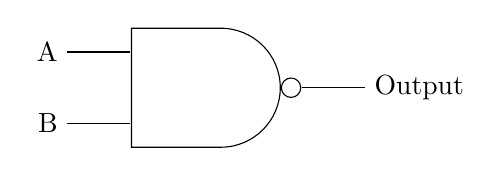
\begin{tikzpicture}[circuit logic US, scale=2]

	\node [nand gate, inputs=nnnn] (nand1) at (0, 0) {};

	\draw (nand1.input 1) -- node[at end, left]{A} ++(left: 4mm);
	\draw (nand1.input 4) -- node[at end, left]{B} ++(left: 4mm);
	\draw (nand1.output) -- node[at end, right]{Output} ++(right: 4mm);

\end{tikzpicture}
\end{center}

\nl
Tablica prawdy (zależności wartości wyjścia bramki od wartości wejść):

{
\centering
\begin{center}
\begin{tabular}{ | c | c | c | } 
  \hline
  \ \ \ \textbf{A} \ \ \ & \ \ \ \textbf{B} \ \ \ & \textbf{Output} \\ 
  \hline
  0 & 0 & 1 \\
  \hline
  0 & 1 & 1 \\
  \hline
  1 & 0 & 1 \\
  \hline
  1 & 1 & 0 \\
  \hline
\end{tabular}
\end{center}
}

\newpage
\paragraph{NOR \\}

Bramka NOR z wejściami \textit{A} i \textit{B} realizuje funkcję NOT-OR, czyli 

$$ NOT \ ( \ \textit{A} \ OR \ \textit{B} \ ) $$

\nl
Oznaczenie bramki NOR w schematach układów logicznych:
\begin{center}
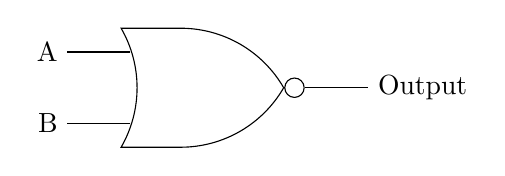
\begin{tikzpicture}[circuit logic US, scale=2]

	\node [nor gate, inputs=nnnn] (nor1) at (0, 0) {};

	\draw (nor1.input 1) -- node[at end, left]{A} ++(left: 4mm);
	\draw (nor1.input 4) -- node[at end, left]{B} ++(left: 4mm);
	\draw (nor1.output) -- node[at end, right]{Output} ++(right: 4mm);

\end{tikzpicture}
\end{center}

\nl
Tablica prawdy:

{
\centering
\begin{center}
\begin{tabular}{ | c | c | c | } 
  \hline
  \ \ \ \textbf{A} \ \ \ & \ \ \ \textbf{B} \ \ \ & \textbf{Output} \\ 
  \hline
  0 & 0 & 1 \\
  \hline
  0 & 1 & 0 \\
  \hline
  1 & 0 & 0 \\
  \hline
  1 & 1 & 0 \\
  \hline
\end{tabular}
\end{center}
}

\nl
\paragraph{XOR \\}

Bramka XOR (lub EXOR z wejściami \textit{A} i \textit{B} realizuje funkcję EXCLUSIVE-OR, czyli 

$$ ( \ \textit{A} \ OR \ \textit{B} \ ) \ AND \ ( \ NOT \ ( \ \textit{A} \ AND \ \textit{B} \ ) \ ) $$

\nl
Oznaczenie bramki XOR w schematach układów logicznych:
\begin{center}
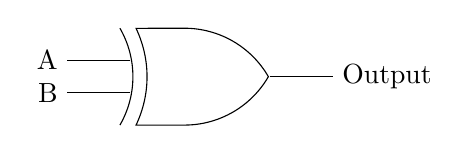
\begin{tikzpicture}[circuit logic US, scale=2]

	\node [xor gate] (xor1) at (0, 0) {};

	\draw (xor1.input 1) -- node[at end, left]{A} ++(left: 4mm);
	\draw (xor1.input 2) -- node[at end, left]{B} ++(left: 4mm);
	\draw (xor1.output) -- node[at end, right]{Output} ++(right: 4mm);

\end{tikzpicture}
\end{center}

\nl
Tablica prawdy:

{
\centering
\begin{center}
\begin{tabular}{ | c | c | c | } 
  \hline
  \ \ \ \textbf{A} \ \ \ & \ \ \ \textbf{B} \ \ \ & \textbf{Output} \\ 
  \hline
  0 & 0 & 0 \\
  \hline
  0 & 1 & 1 \\
  \hline
  1 & 0 & 1 \\
  \hline
  1 & 1 & 0 \\
  \hline
\end{tabular}
\end{center}
}

\newpage
Elektronicznie bramki logiczne realizowane są za pomocą tranzystorów (elementów elektronicznych mogących pełnić rolę przełącznika sterowanego napięciem). Z historycznego punktu widzenia to właśnie użycie półprzewodników do budowy tranzystorów najmocniej pchnęło do przodu rozwój komputerów. Wcześniej układy logiczne budowano przy użyciu lamp próżniowych. Użycie tranzystorów półprzewodnikowych pozwoliło zmniejszyć rozmiary i efektywność bramek logicznych, a co za tym idzie procesorów i układów pamięci. Dla przykładu poniżej zamieszczam schemat bramki NAND realizowanej przy pomocy tranzystorów typu NPN: \\

\begin{center}
\begin{circuitikz}[scale=1.2]

  	\draw (0,0) node[npn] (npn1) {};
	\draw ($(npn1)-(0.1,0)$) circle [radius=18pt];

	\draw (0,-3) node[npn] (npn2) {};
	\draw ($(npn2)-(0.1,0)$) circle [radius=18pt];

	\draw (npn1.emitter) to (npn2.collector);

	\draw (npn2.emitter) to (0,-5) node[ground]{};

	\draw (npn1.collector) to (0,1)
				to [R=$R_1$] (0,4.5)
				to (0,4.6) node[vcc]{$V_{cc}$};

	\draw (0,1) to [short,-o] (4, 1) node[anchor=south]{Y};

	\draw (npn1.base) to (-1,0)
				to [R=$R_2$] (-4,0)
				to [short,-o] (-5,0) node[anchor=south]{A};

	\draw (npn2.base) to (-1,-3)
				to [R=$R_2$] (-4,-3)
				to [short,-o] (-5,-3) node[anchor=south]{B};

\end{circuitikz}
\end{center}

\nl 
Tylko w przypadku, kiedy napięcie będzie podane na obydwa wejścia A i B obydwa tranzystory będą "zamknięte", pozwalając napięciu z zasilania ($V_{cc}$) płynąć prosto do masy. W innym przypadku napięcie z zasilania jest obserwowane na wyjściu Y.

\newpage
\paragraph{Ćwiczenie 4.1 \\}
Zapoznanie się z płytką UC-2 do badania układów z scalonych TTL.

\begin{figure}[H]
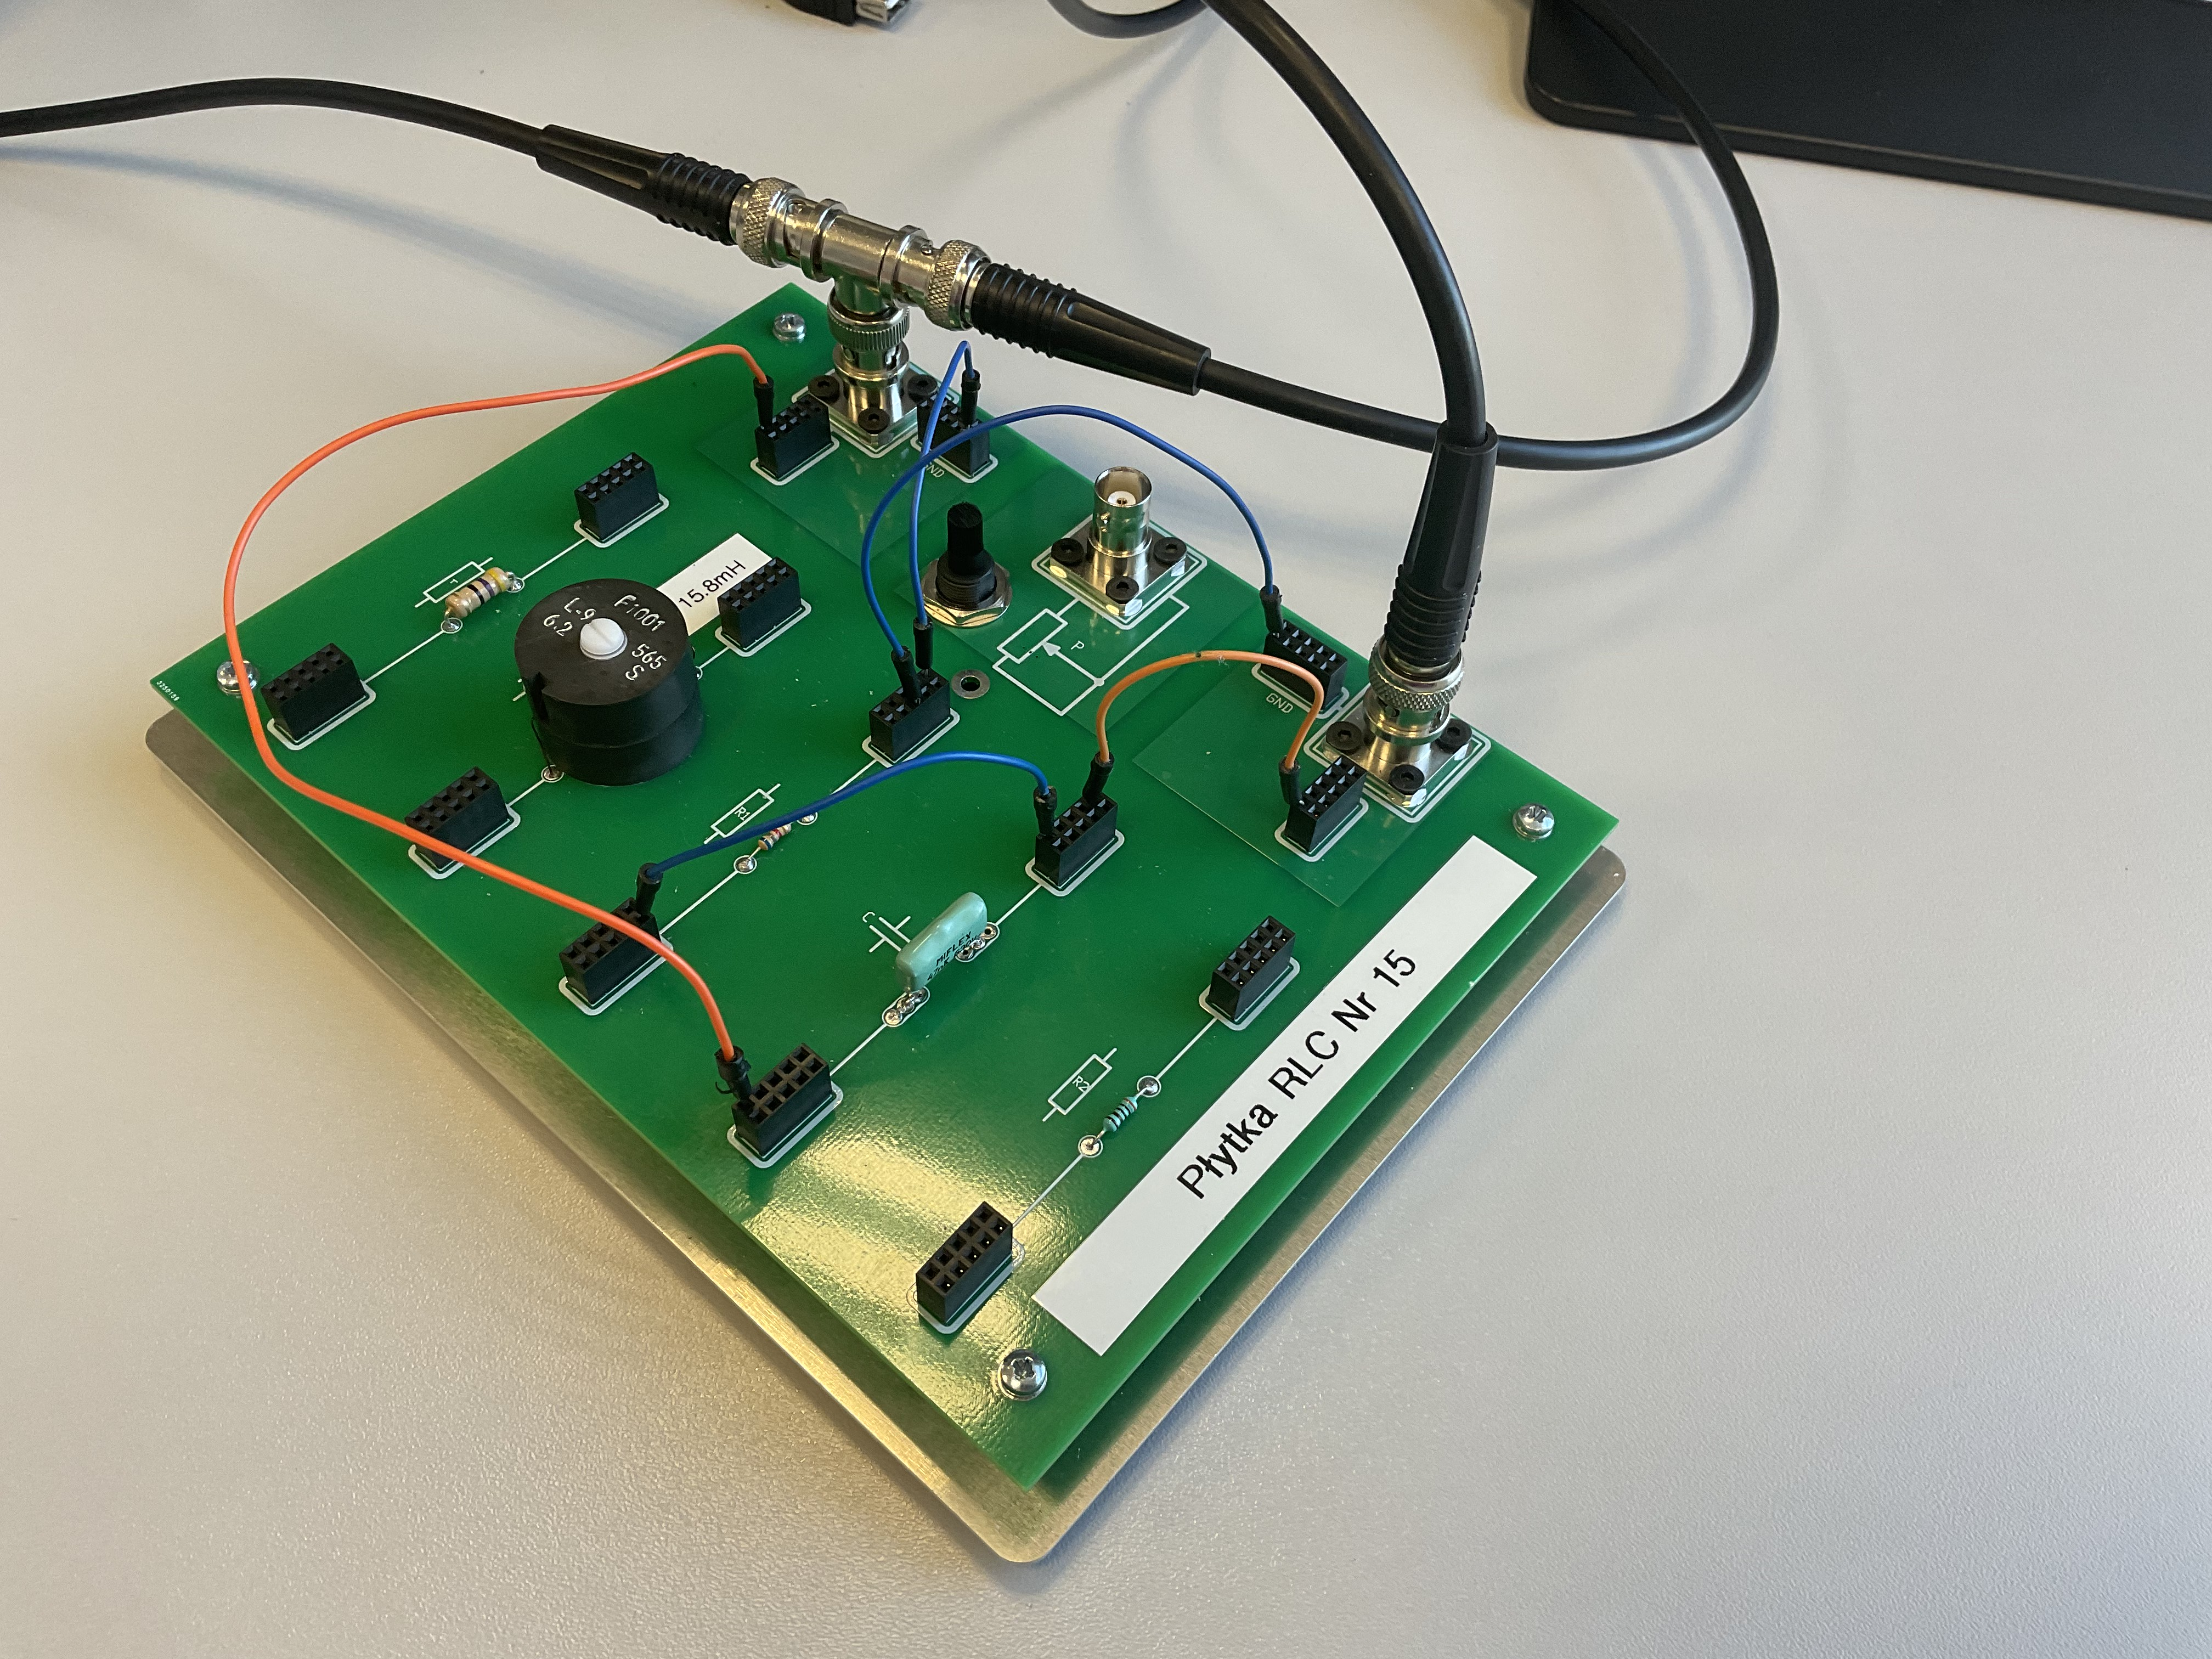
\includegraphics[scale=0.07]{C0}
\centering
\captionsetup{labelformat=empty}
\caption{Płytka UC-2.}
\end{figure}

Na płytce znajdują się dwa impulsatory do wytwarzania sygnałów logicznych, próbnik stanów logicznych (komparator do sprawdzania wartości logicznej sygnału), osiem diod, dwa złącza BNC oraz dwa gniazda na układy scalone: 16-pinowe i 14-pinowe. Obok gniazd znajdują się także piny zasilające ($5 \ V$) oraz masy ($0 \ V$). \\

\newpage
Zmierzyłem napięcia na pinach $5 \ V$ oraz na wyjściach impulsatorów. Każdy impulsator ma wyjście $Q$ oraz wyjście zaprzeczone $\overline{Q}$. Na wyjście $Q$ w stanie domyślnym podane jest $0 \ V$ (logiczny stan fałszu - FALSE), a na wyjście $\overline{Q}$ - $5 \ V$ (logiczny stan prawdy - TRUE). Naciśnięcie przycisku powoduje zamianę stanów - $Q$ na TRUE i $\overline{Q}$ na FALSE.

\begin{figure}[H]
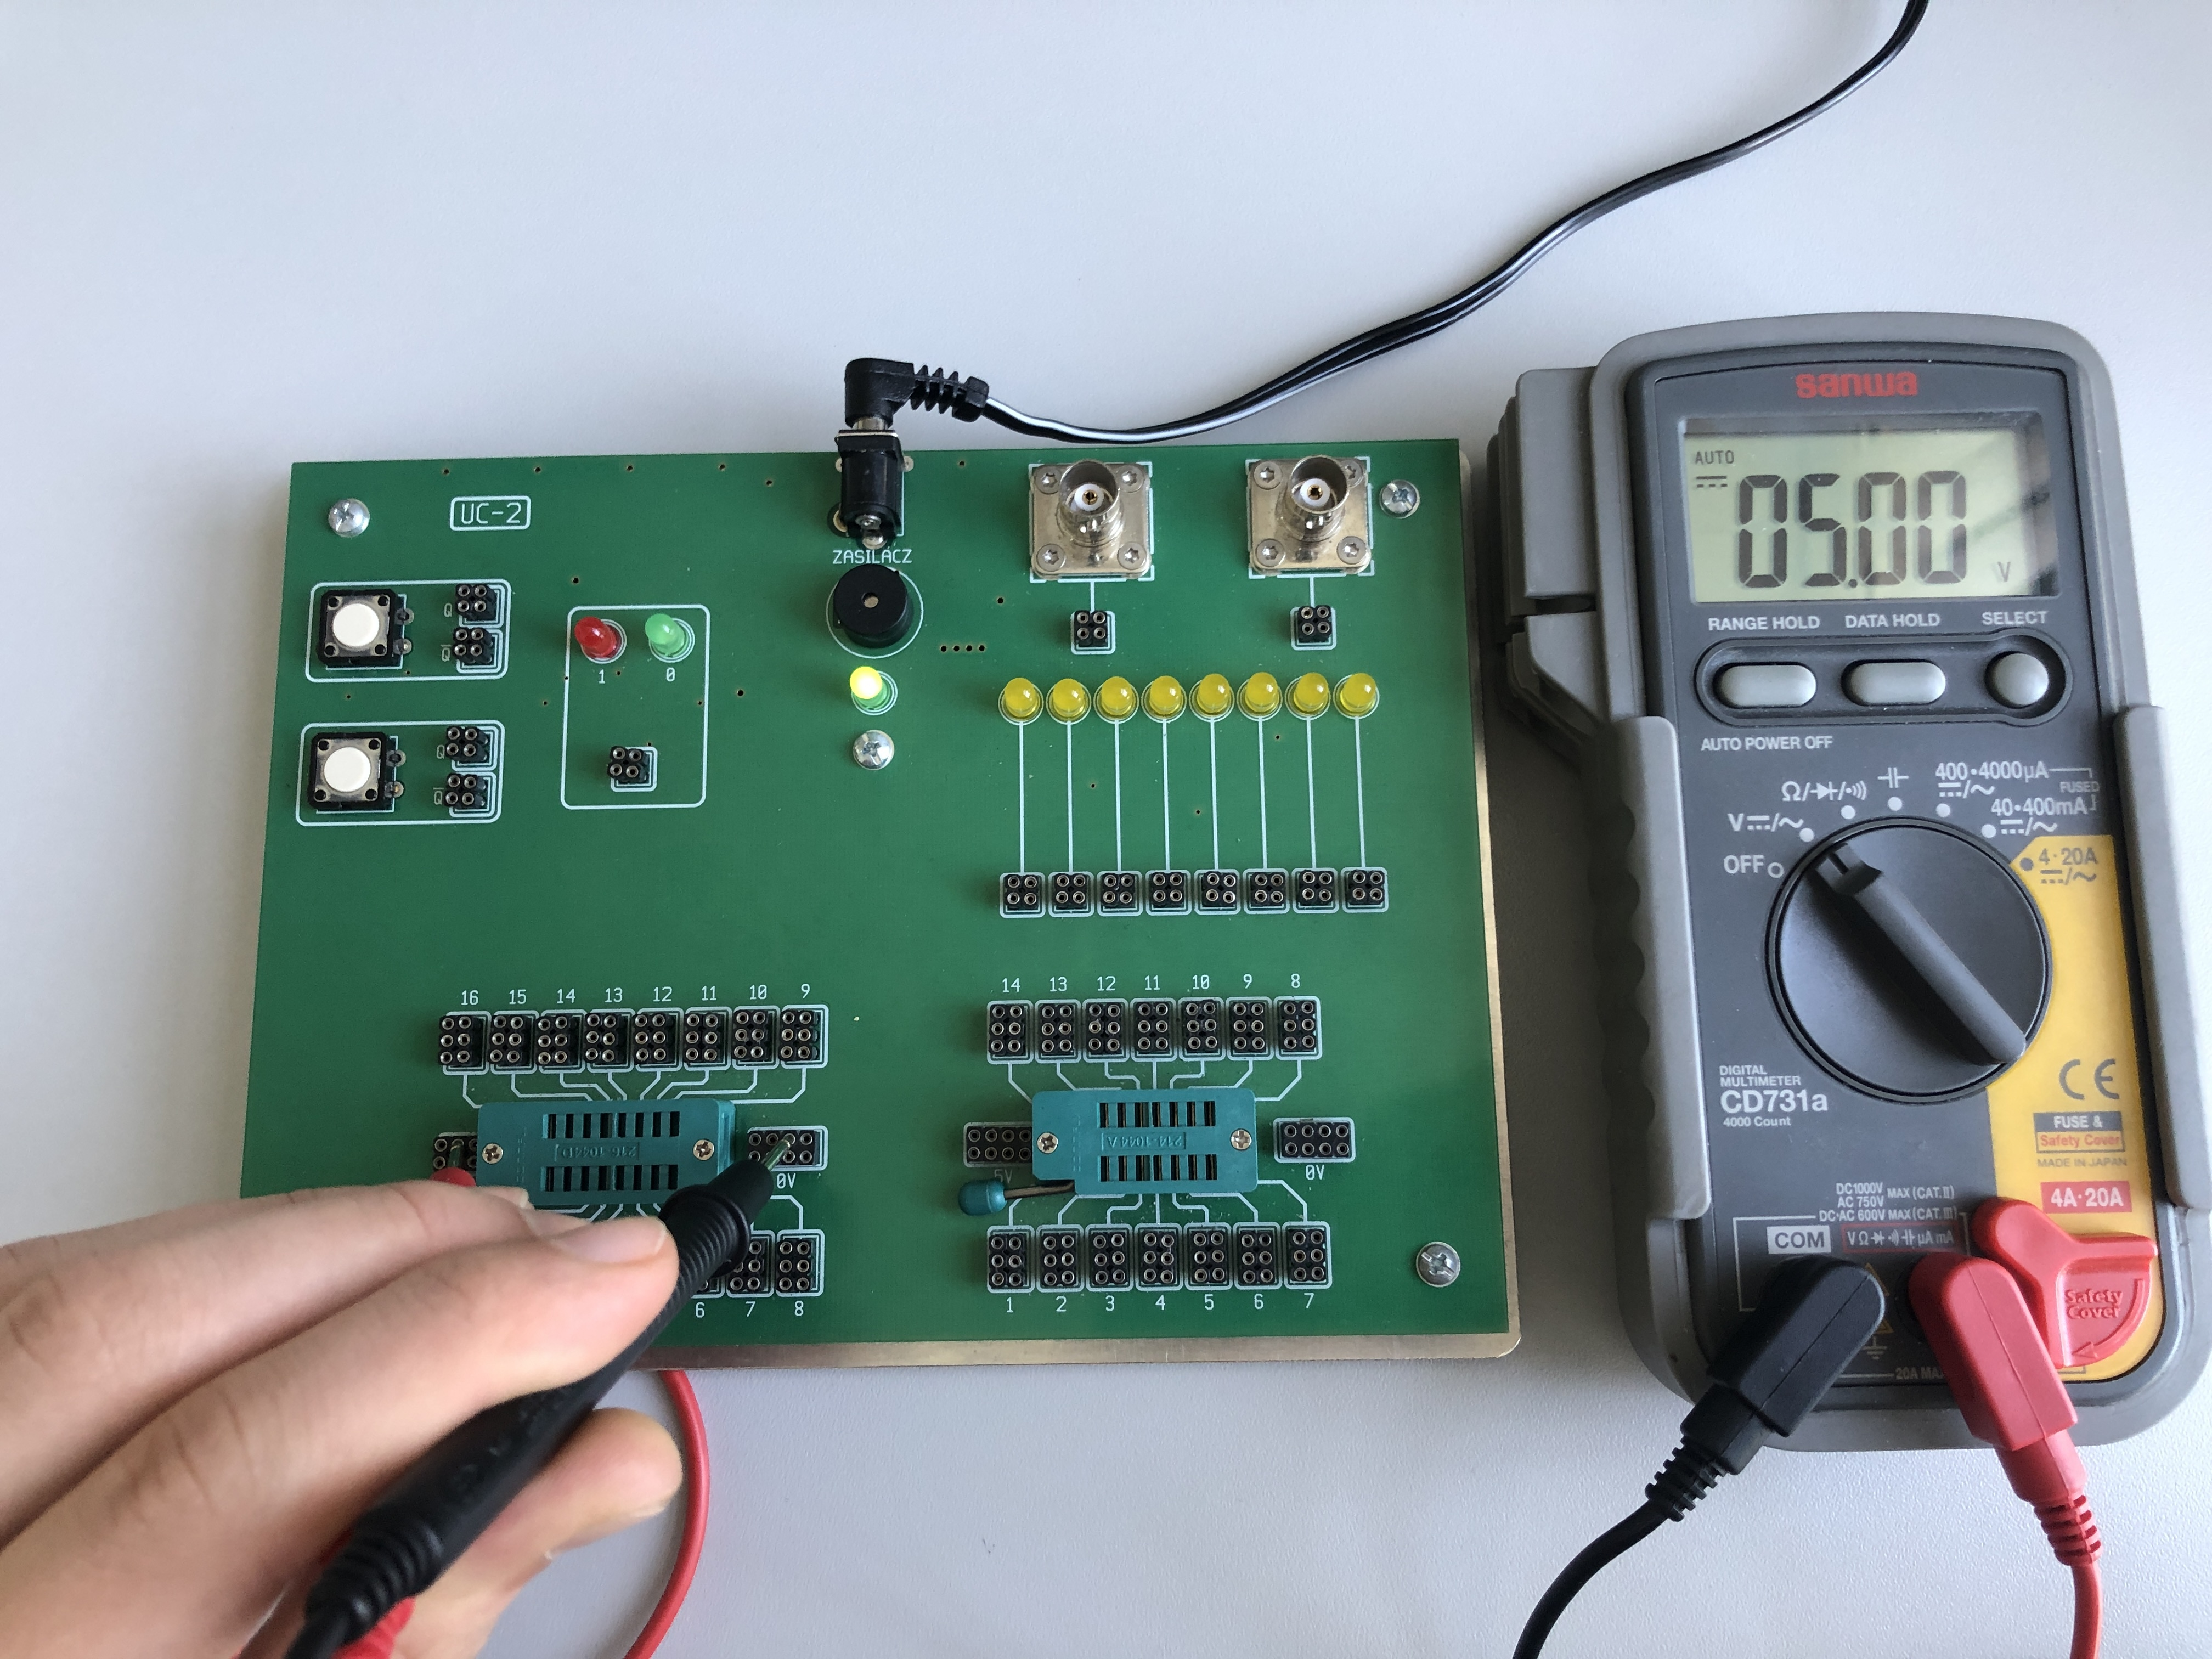
\includegraphics[width=7cm]{C62}
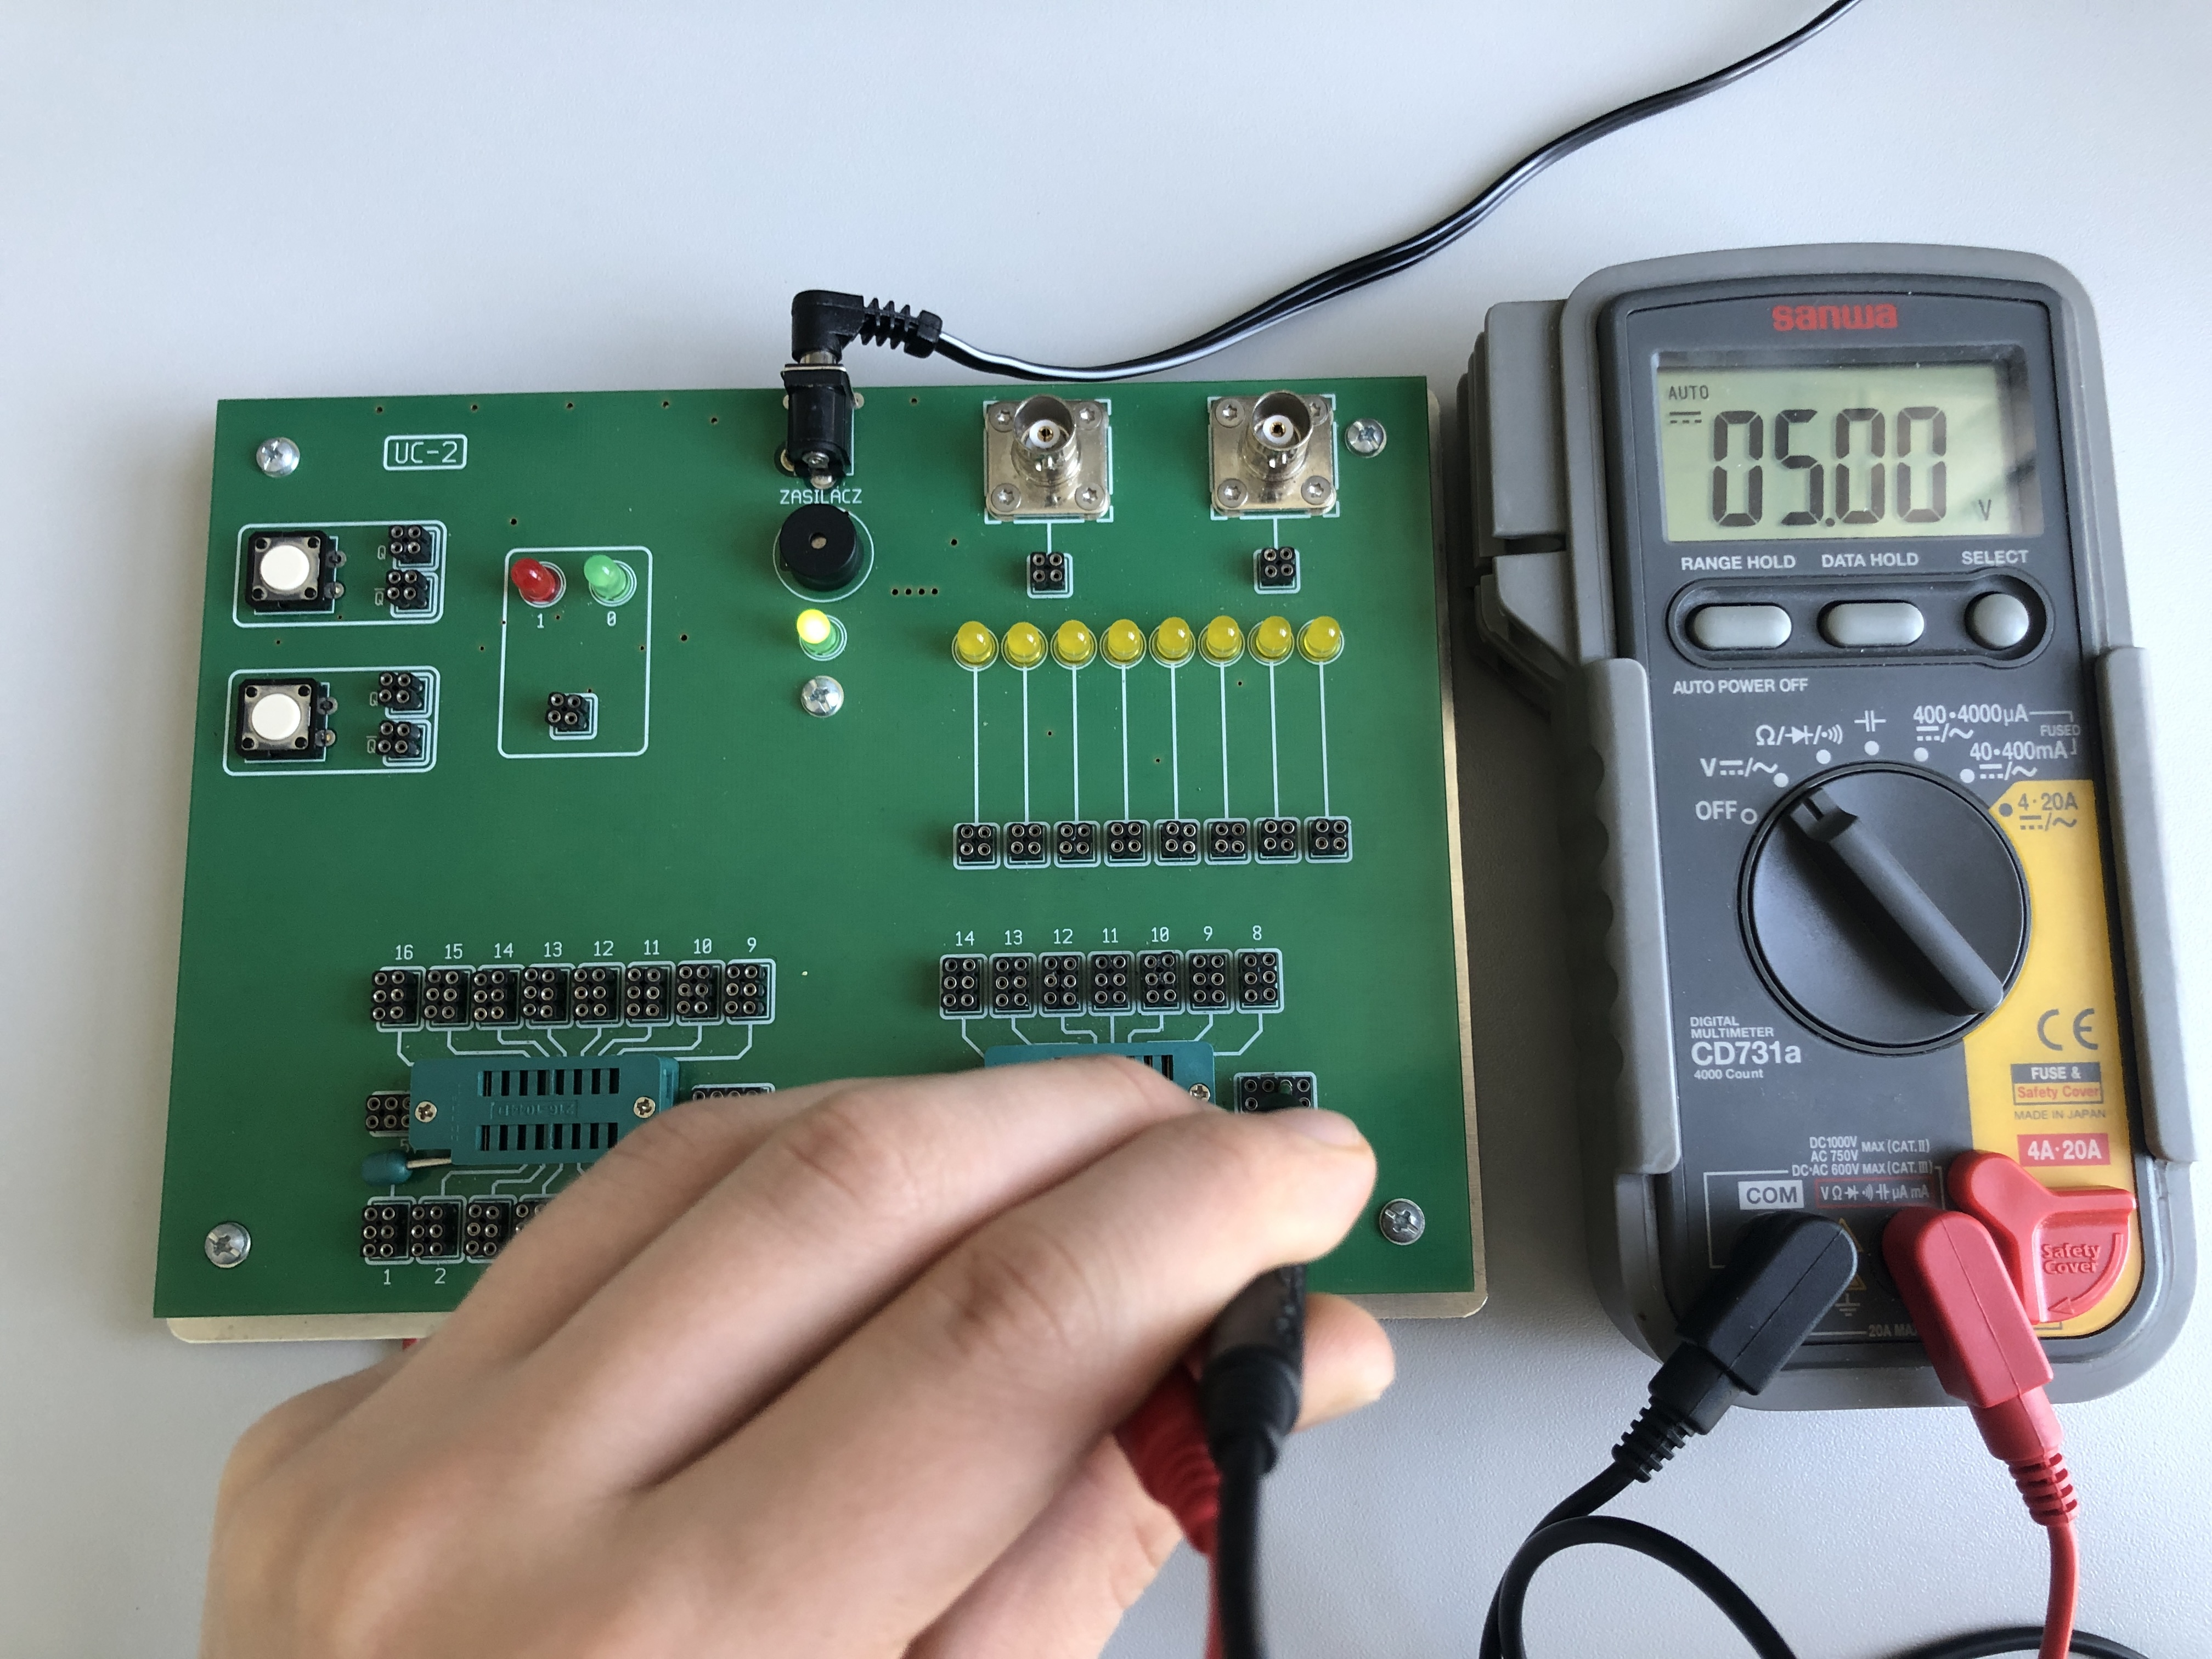
\includegraphics[width=7cm]{C63}
\centering
\captionsetup{labelformat=empty}
\caption{Napięcia $5 \ V$}
\end{figure}

\begin{figure}[H]
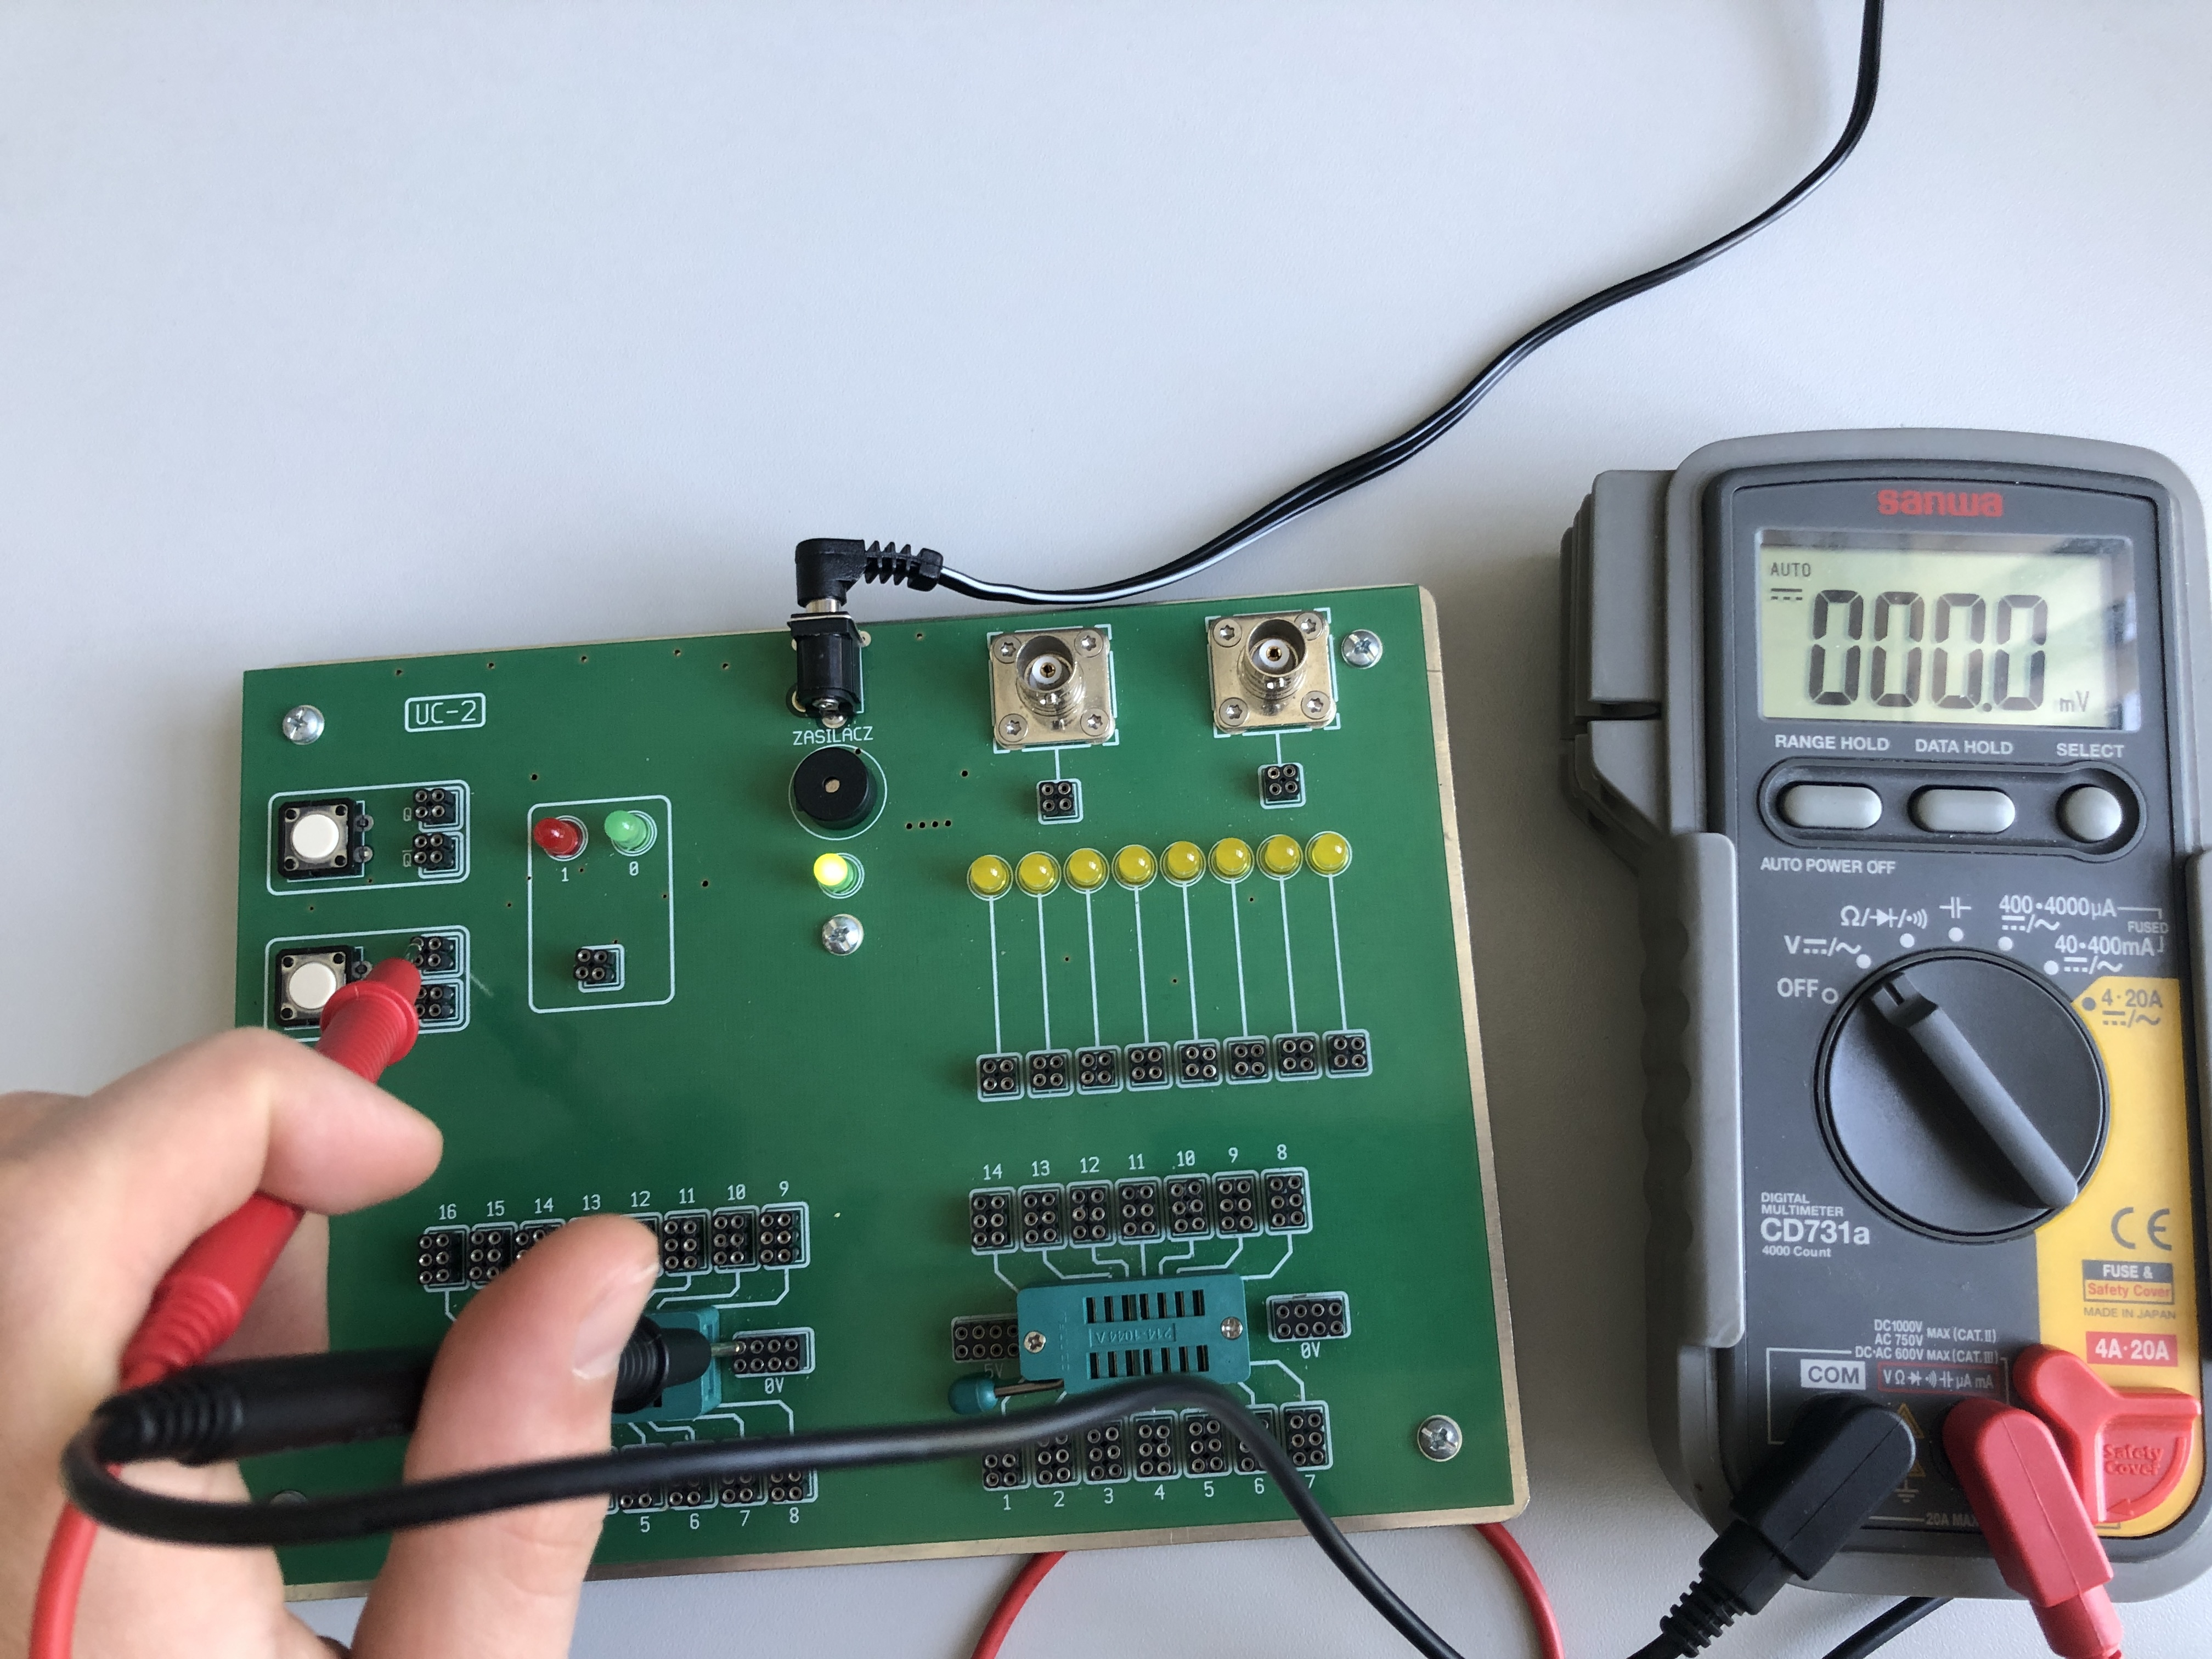
\includegraphics[width=7cm]{C65}
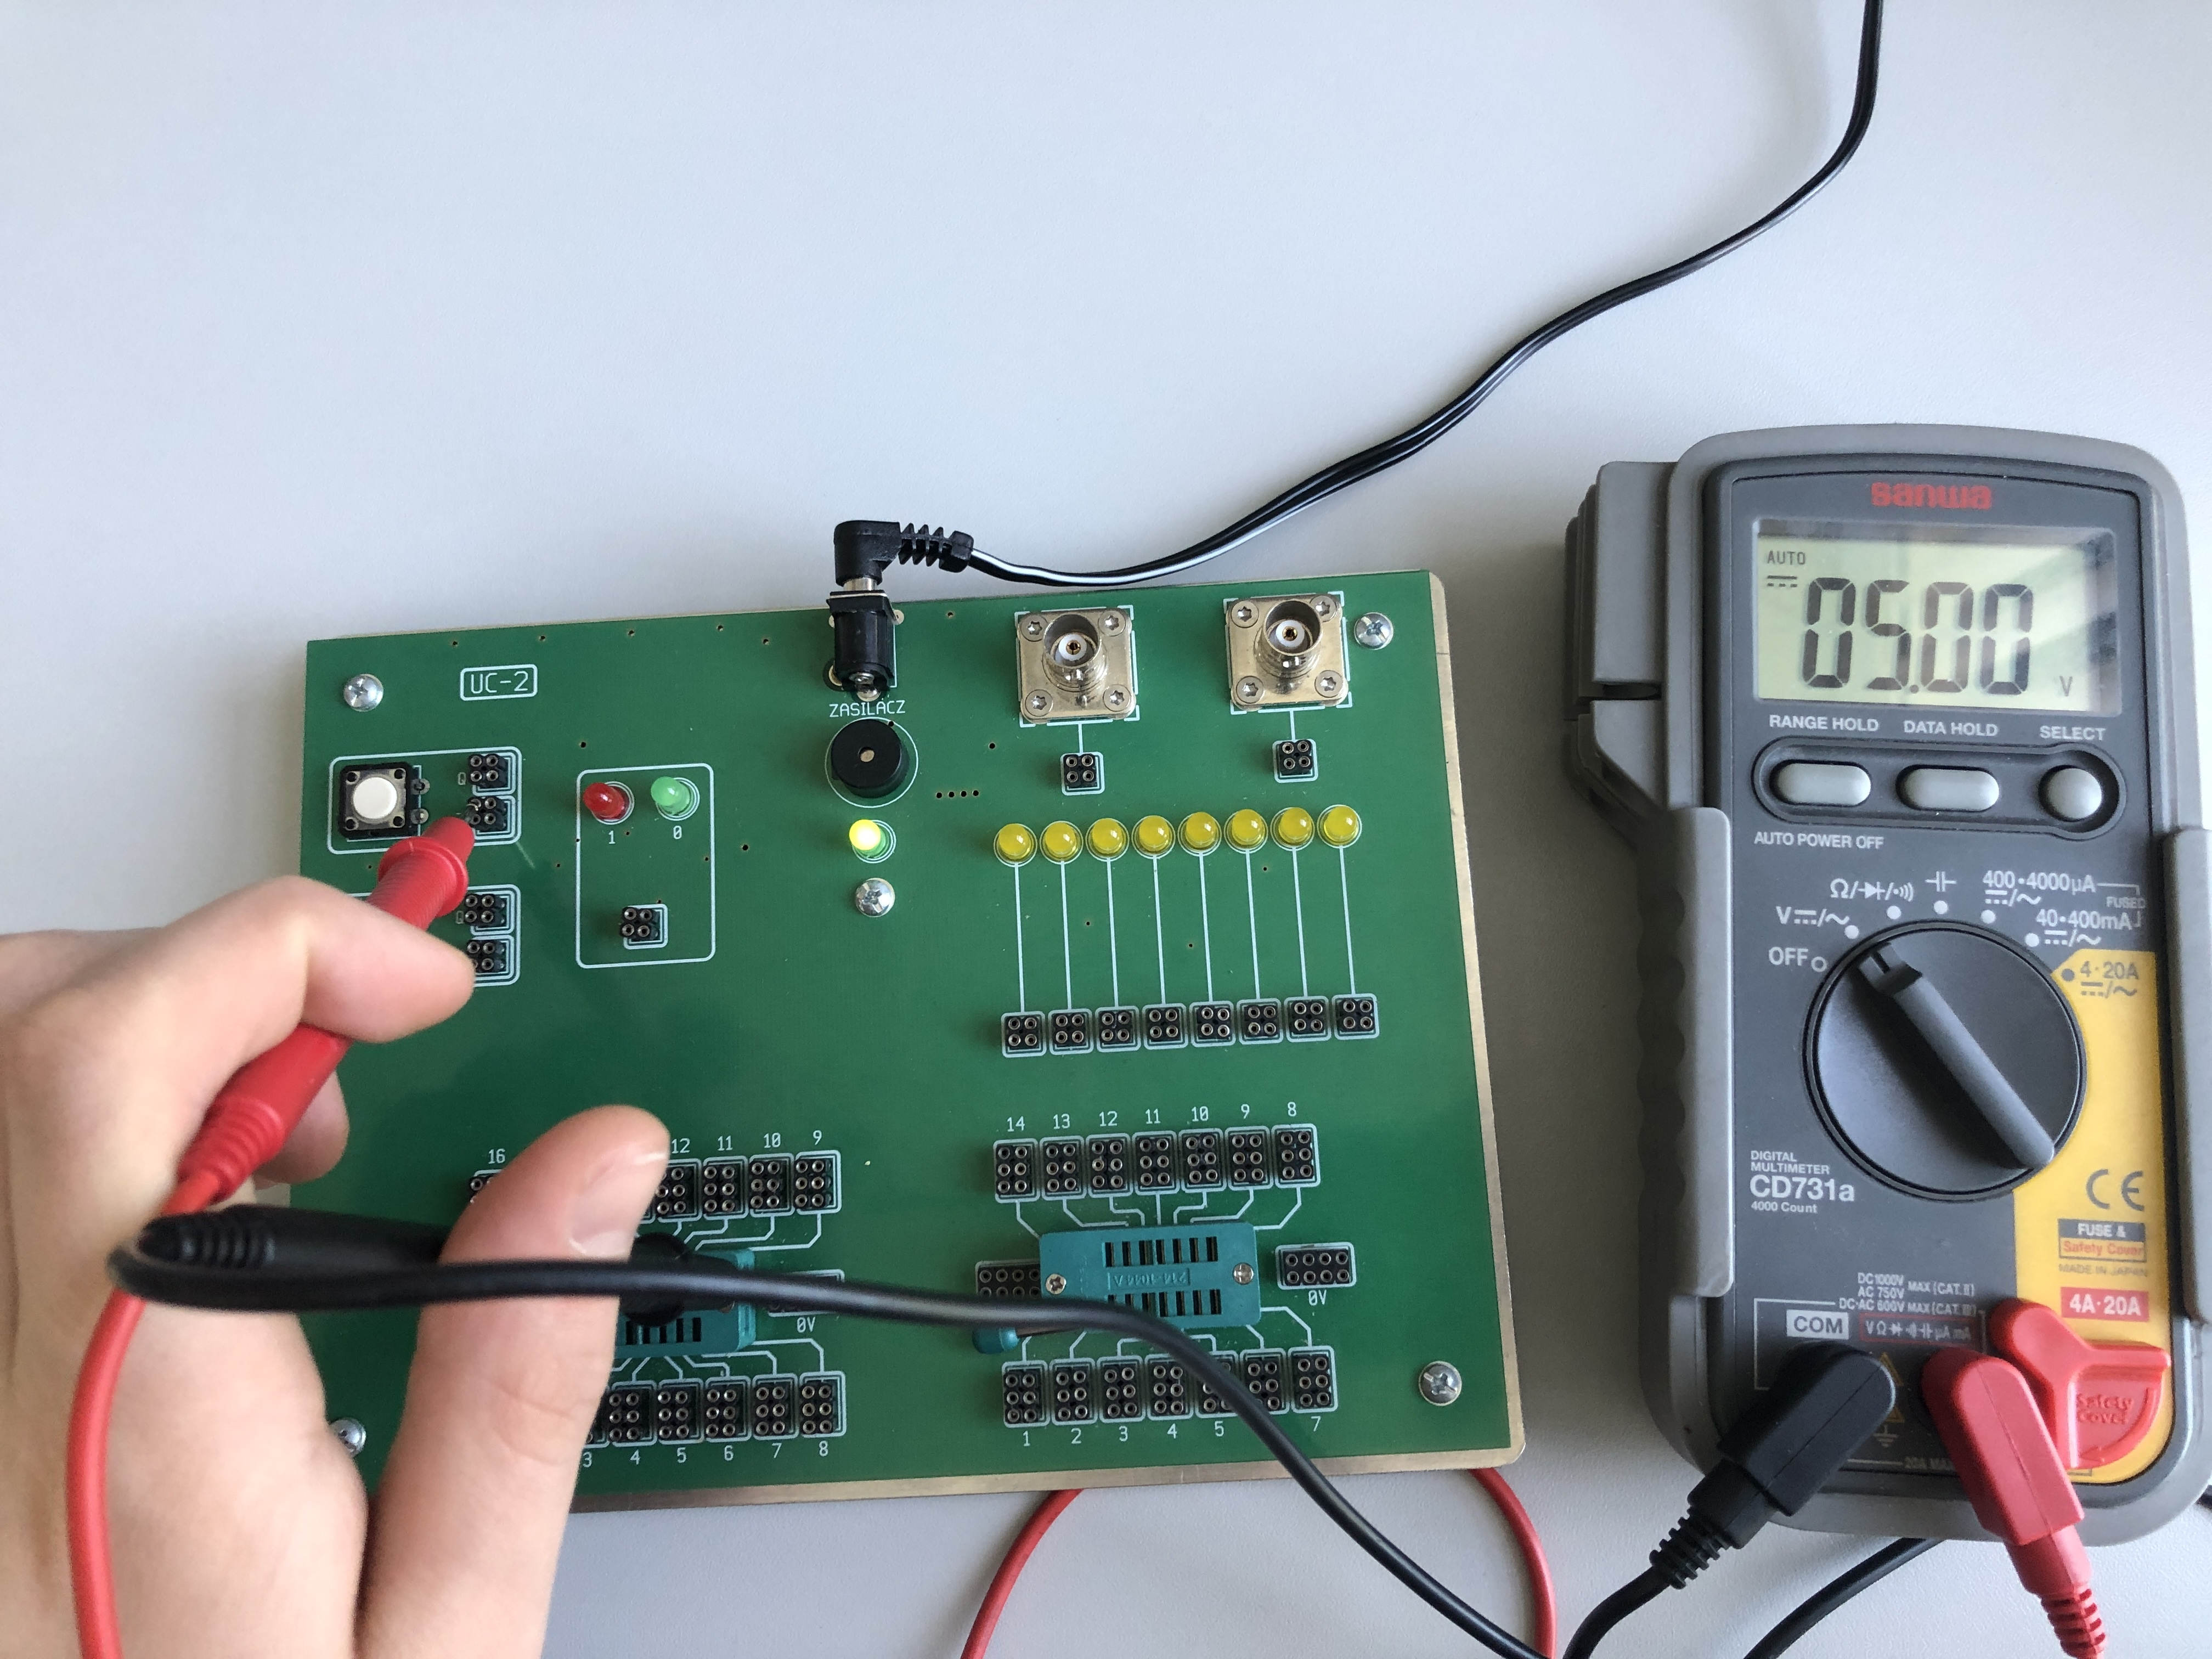
\includegraphics[width=7cm]{C64}
\centering
\captionsetup{labelformat=empty}
\caption{Wyjścia $Q$ oraz $\overline{Q}$ impulsatora}
\end{figure}

\begin{figure}[H]
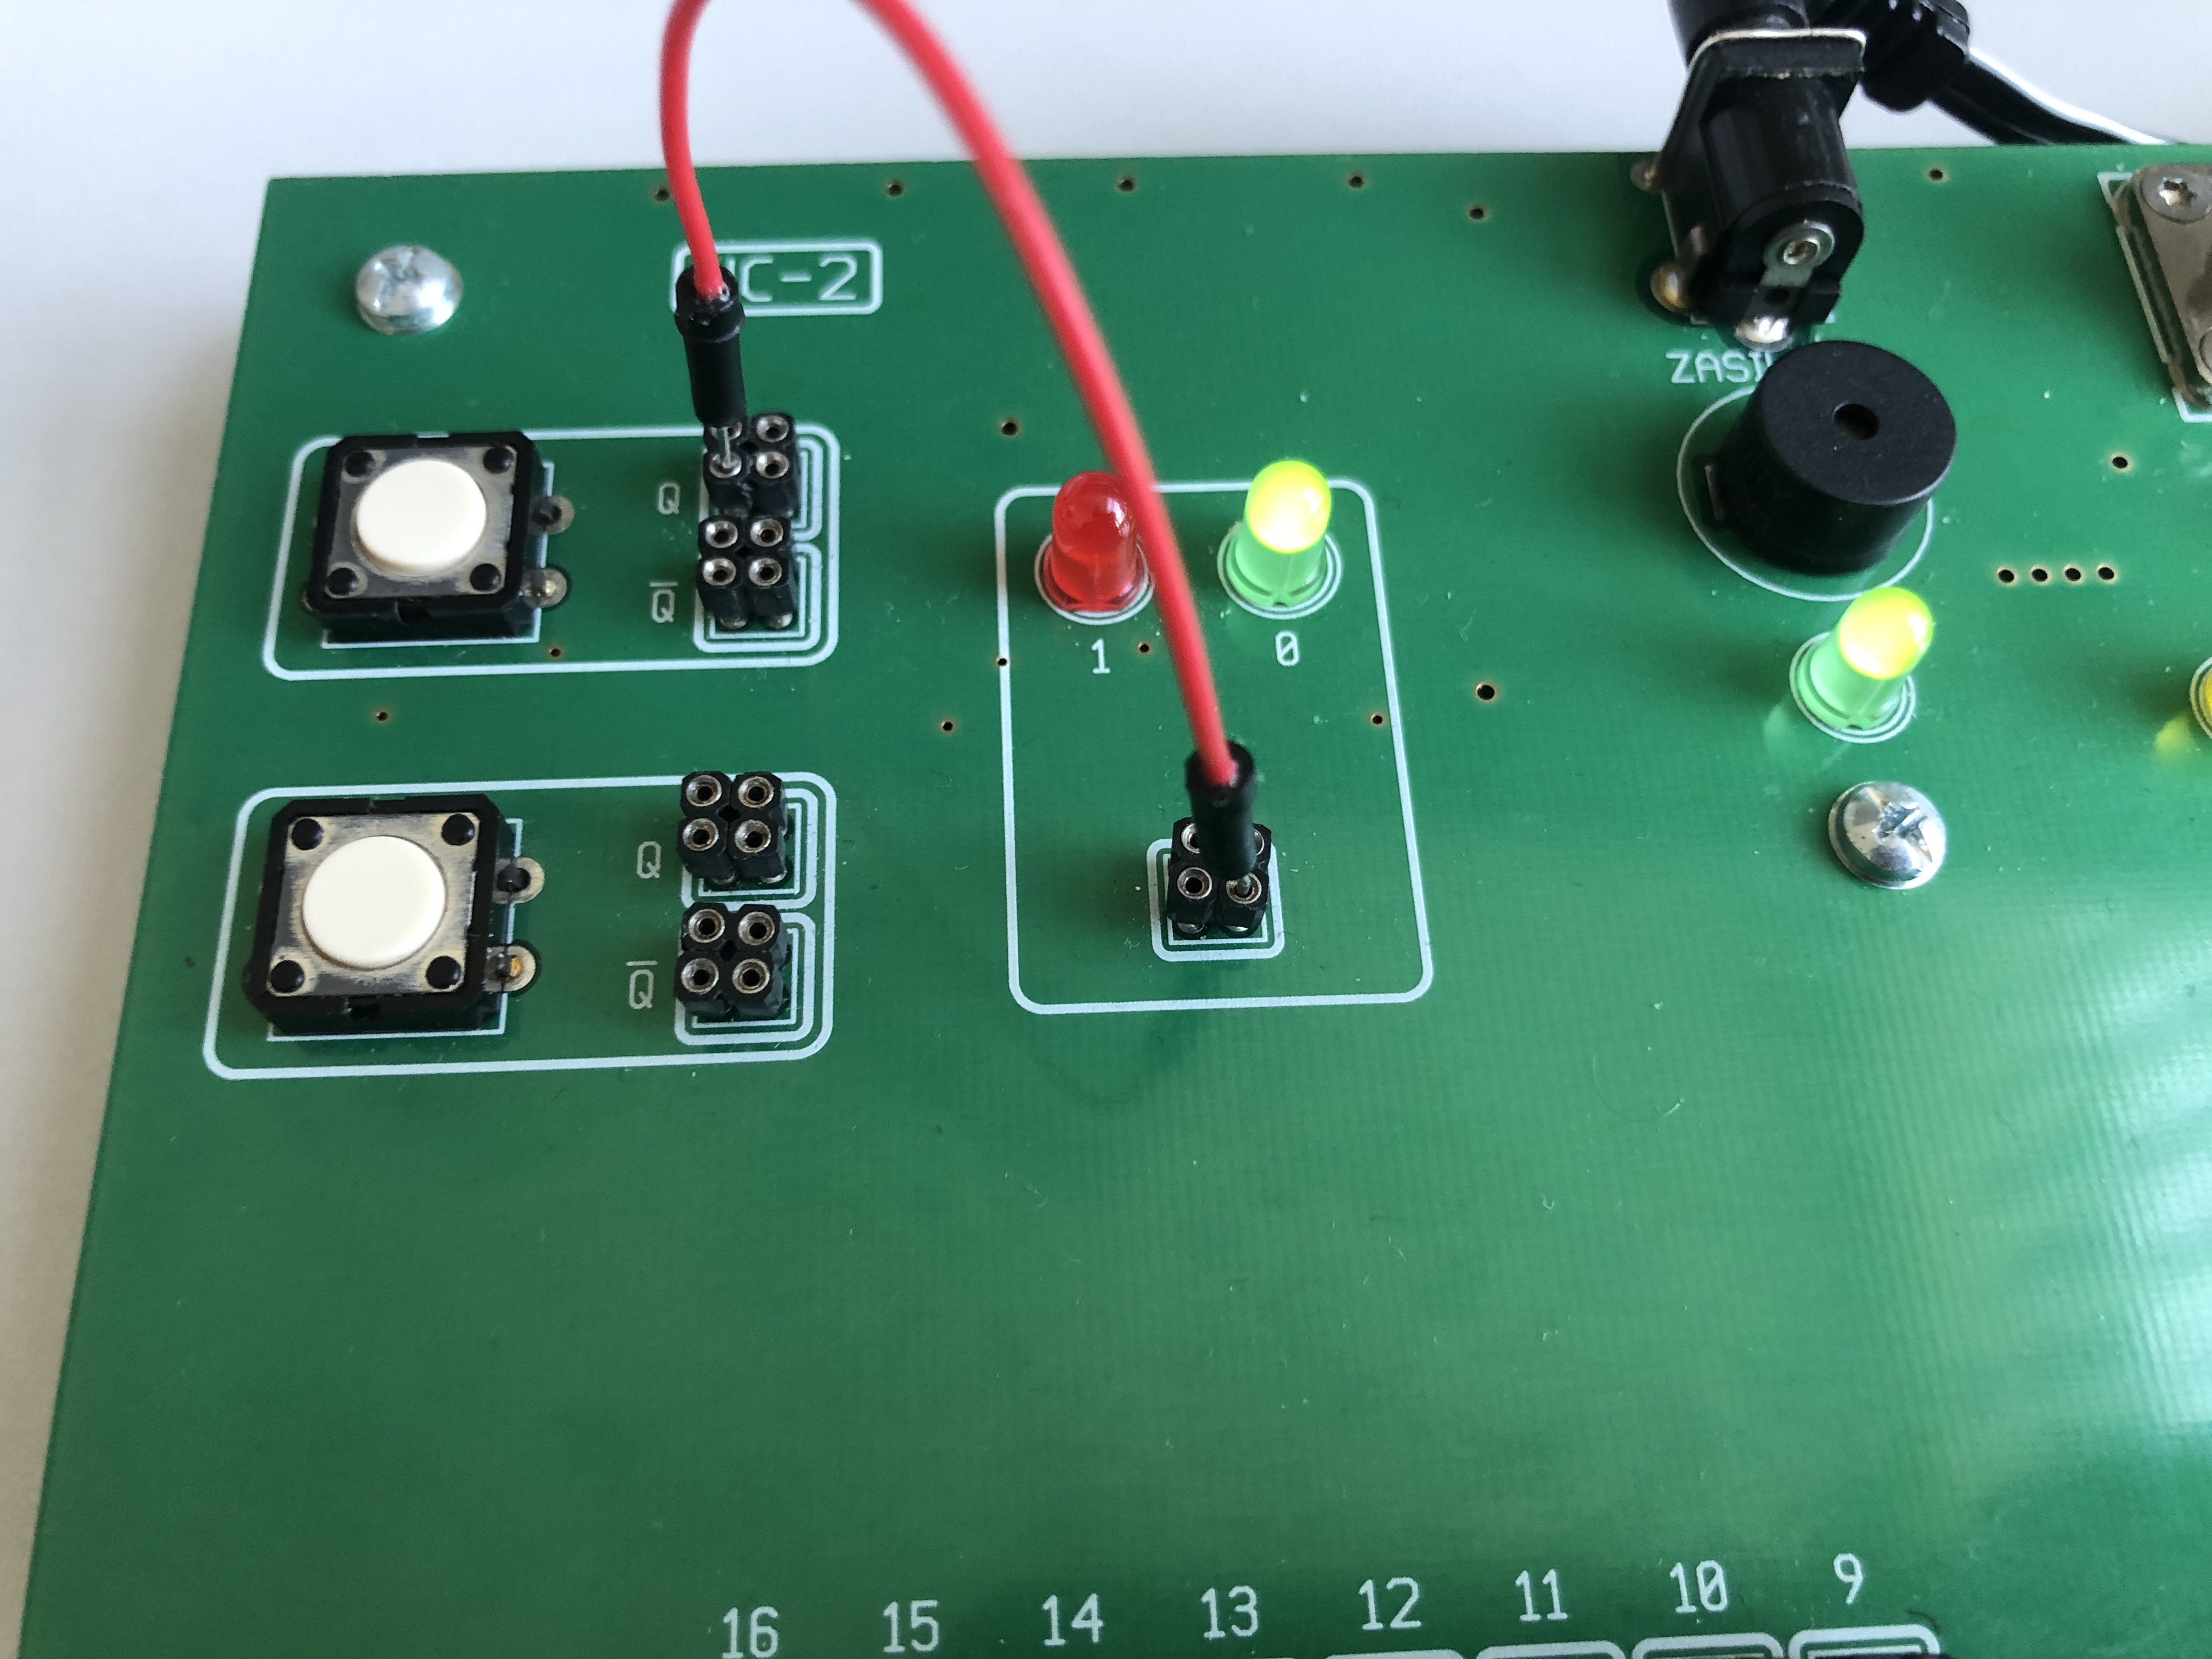
\includegraphics[width=7cm]{C66}
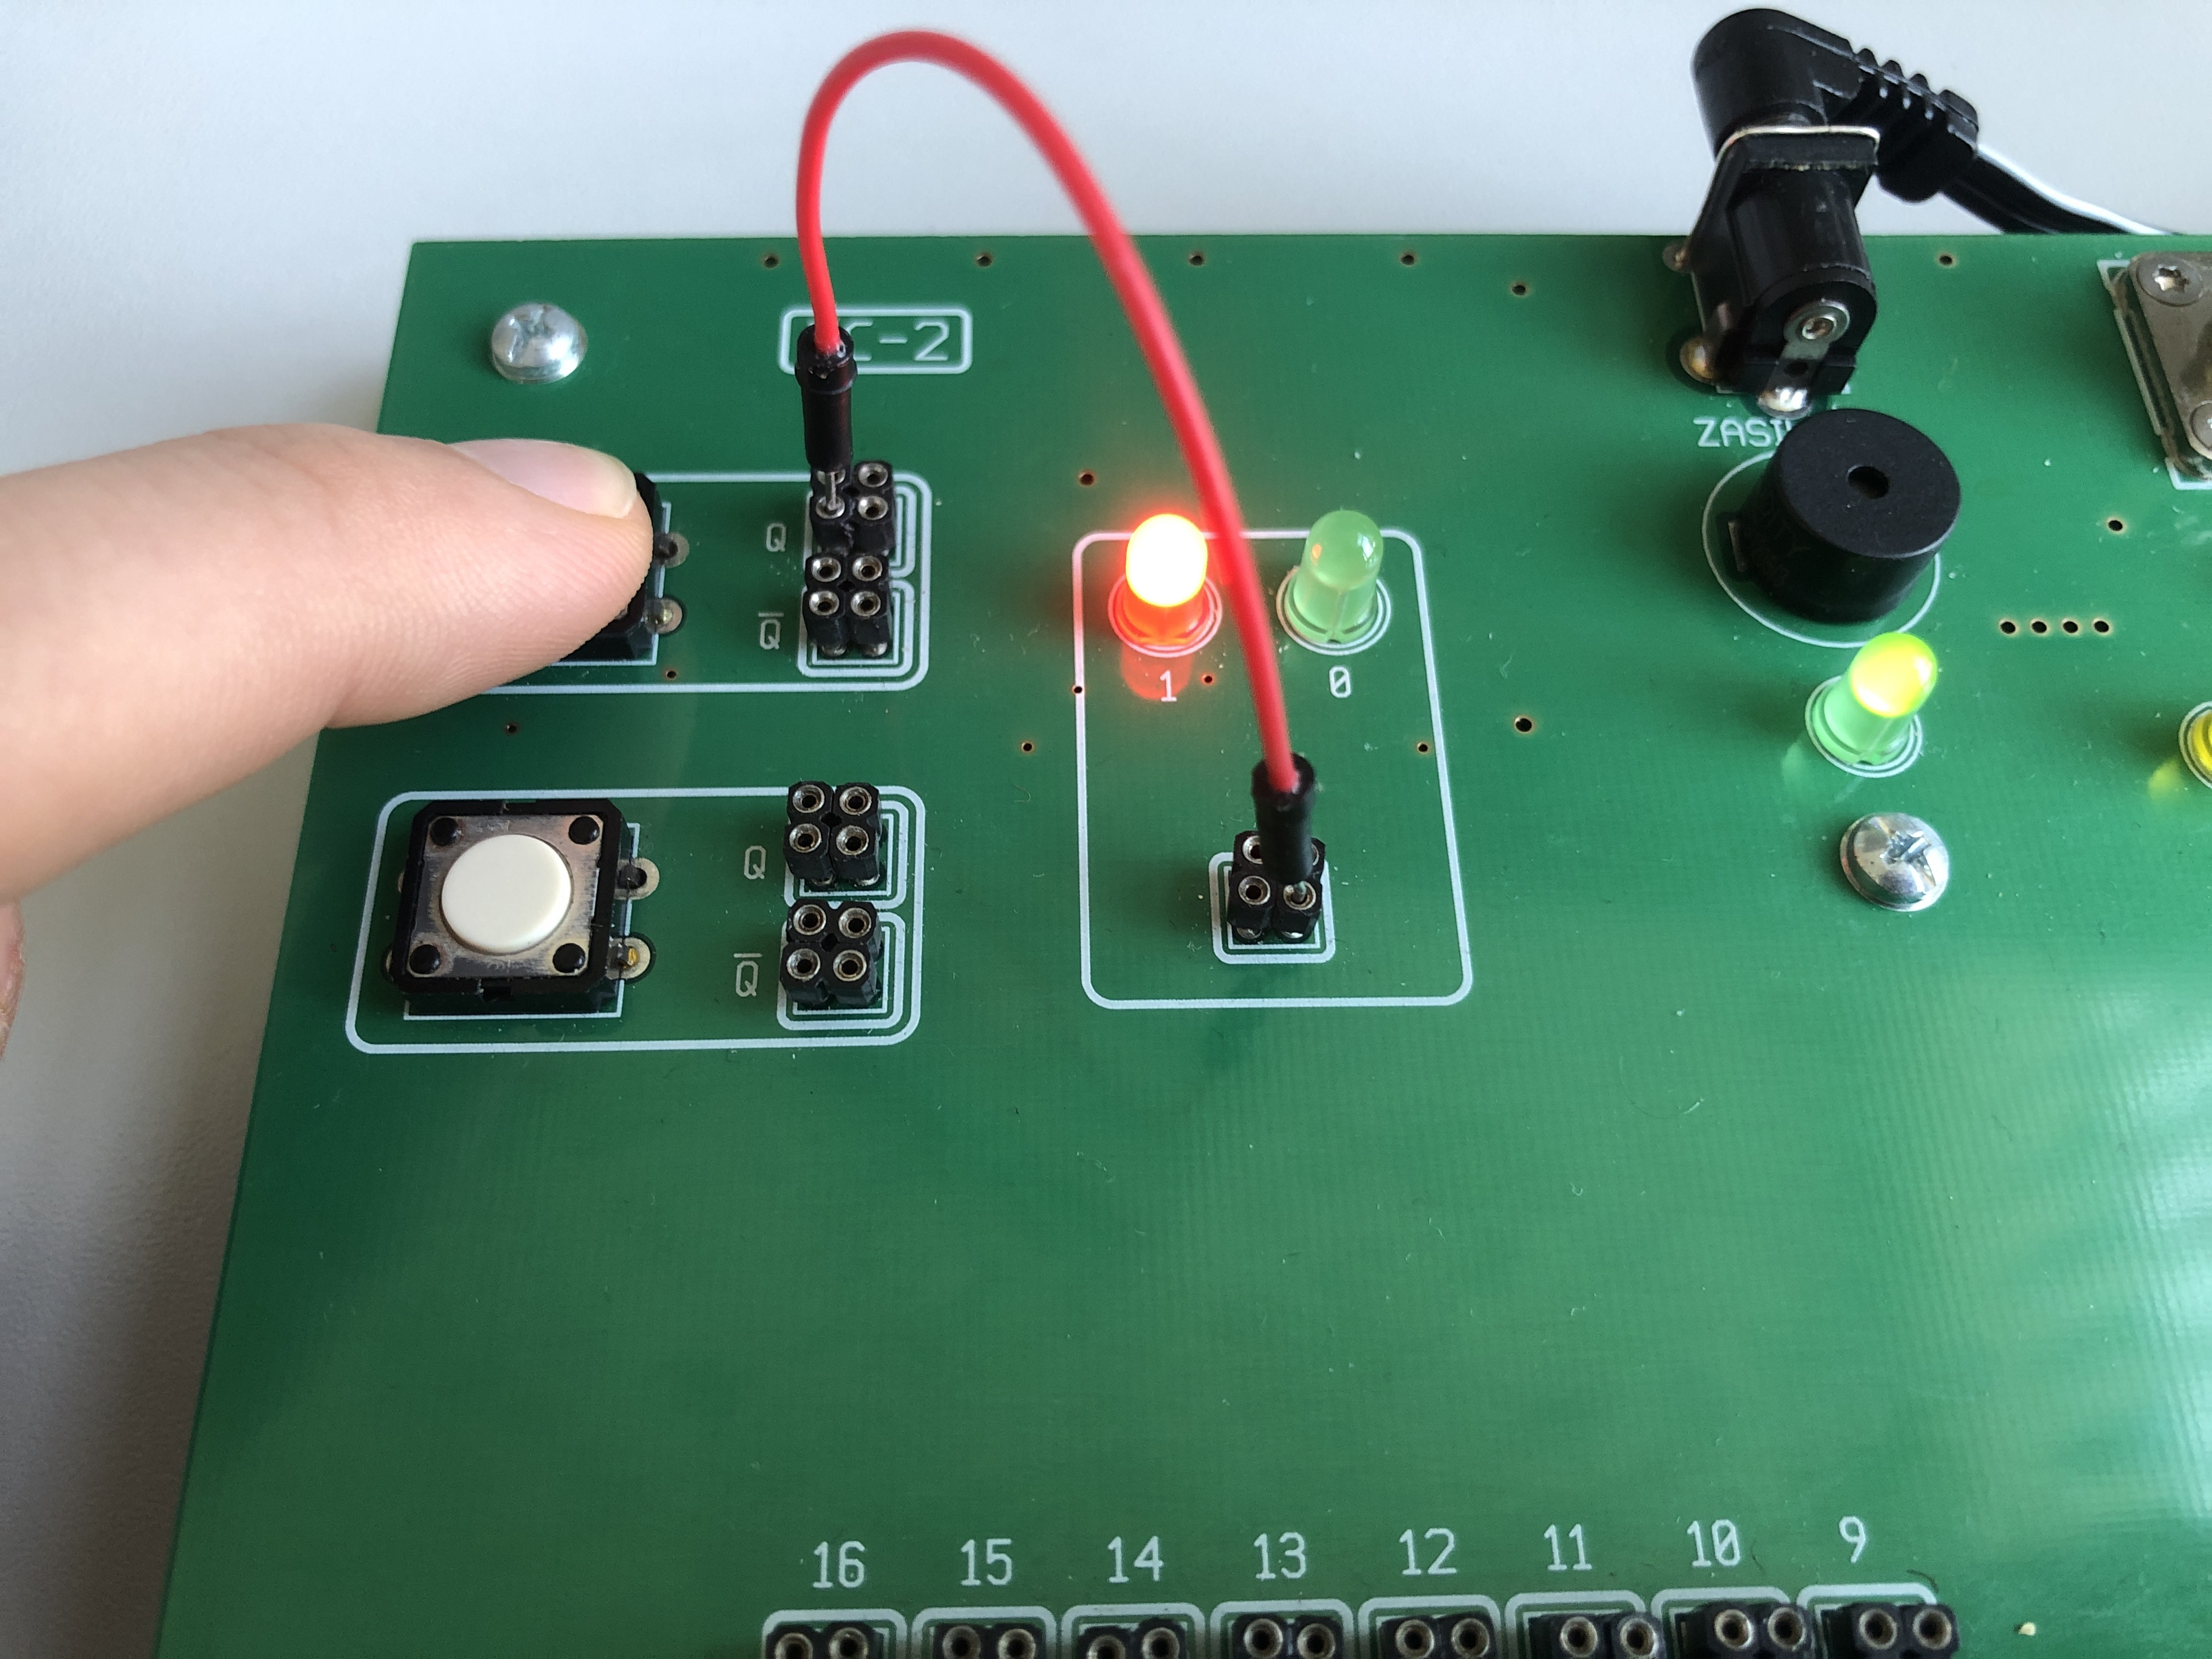
\includegraphics[width=7cm]{C67}
\centering
\captionsetup{labelformat=empty}
\caption{Sygnały logiczne: 0 (FALSE) oraz 1 (TRUE) na wyjściu $Q$ impulsatora}
\end{figure}

\newpage
\paragraph{Ćwiczenie 4.2 \\}
Zbadanie tablicy logicznej dla bramek logicznych NAND, NOR i XOR mierząc poziomy napięć na ich wyjściach i sprawdzając je próbnikiem stanów logicznych. \\

W 14-pinowe gniazdo na płytce UC-2 wpiąłem układy 7400 (NAND), 7402 (NOR) oraz 7486 (XOR). Na wejścia każdej z bramek podałem wyjścia $Q$ (sygnał $0$ albo $5\ V$) obydwu impulsatorów i zmieniając stany wyjść $Q$ mierzyłem napięcie na wyjściach bramek. \\

Zmierzone przeze mnie napięcia podane są w tabelach poniżej. \\

{
\centering
\begin{center}
\begin{tabular}{ | c | c | c | } 
  \hline
  \ \ \ \textbf{A} \ \ \ & \ \ \ \textbf{B} \ \ \ & \textbf{A NAND B} \\ 
  \hline
  $0 \ V$ & $0 \ V$ & $4.16 \ V$ \\
  \hline
  $0 \ V$ & $5 \ V$ & $4.16 \ V$ \\
  \hline
  $5 \ V$ & $0 \ V$ & $4.16 \ V$ \\
  \hline
  $5 \ V$ & $5 \ V$ & $400 \ mV$ \\
  \hline
\end{tabular}
\end{center}
}

\nl

{
\centering
\begin{center}
\begin{tabular}{ | c | c | c | } 
  \hline
  \ \ \ \textbf{A} \ \ \ & \ \ \ \textbf{B} \ \ \ & \textbf{A NOR B} \\ 
  \hline
  $0 \ V$ & $0 \ V$ & $4.16 \ V$ \\
  \hline
  $0 \ V$ & $5 \ V$ & $400 \ mV$ \\
  \hline
  $5 \ V$ & $0 \ V$ & $320 \ mV$ \\
  \hline
  $5 \ V$ & $5 \ V$ & $320 \ mV$ \\
  \hline
\end{tabular}
\end{center}
}

\nl

{
\centering
\begin{center}
\begin{tabular}{ | c | c | c | } 
  \hline
  \ \ \ \textbf{A} \ \ \ & \ \ \ \textbf{B} \ \ \ & \textbf{A XOR B}\\ 
  \hline
  $0 \ V$ & $0 \ V$ & $320 \ mV$ \\
  \hline
  $0 \ V$ & $5 \ V$ & $5.36 \ V$ \\
  \hline
  $5 \ V$ & $0 \ V$ & $5.28 \ V$ \\
  \hline
  $5 \ V$ & $5 \ V$ & $400 \ mV$ \\
  \hline
\end{tabular}
\end{center}
}

Po zmierzeniu napięć na wyjściach bramek podpiąłem zamiast oscyloskopu próbnik stanów logicznych, który pozwolił mi zweryfikować, że bramki zachowują się zgodnie z przewidywaniami (tak jak w tabelach zamieszczonych w sekcji "Wstęp" w tym dokumencie). Zdjęcia pomiarów oscyloskopu oraz pomiarów próbnikiem stanów logicznych zamieszczam w pliku \texttt{Sprawozdanie-4-Kwinta-Zalacznik-1}, by zmniejszyć rozmiar samego sprawozdania.

\newpage
\paragraph{Ćwiczenie 4.3 a) \\}
Używając tylko funktorów NAND zbudowanie układu realizującego sumę logiczną (OR), iloczyn logiczny (AND) oraz negację (NOT), sprawdzając ich tablice logiczne używając próbnika stanów logicznych.

\begin{center}
\textbf{AND} - iloczyn logiczny \\
\nl
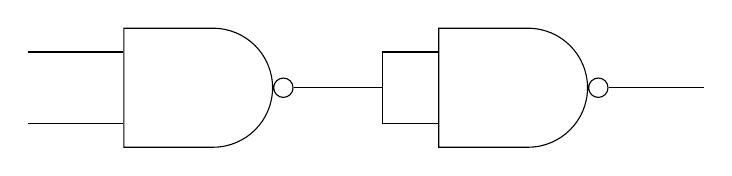
\begin{tikzpicture}[circuit logic US, scale=2]

	\node [nand gate, inputs=nnnn] (gate1) at (0,0) {};
	\node [nand gate, inputs=nnnn] (gate2) at (2,0) {};

	\draw (gate1.output) -- (1.2,0);

	\draw (1.2,0) |- (gate2.input 1);
	\draw (1.2,0) |- (gate2.input 4);

	\draw (gate1.input 1) -- ++(left: 6mm);
	\draw (gate1.input 4) -- ++(left: 6mm);
	\draw (gate2.output) -- ++(right: 6mm);

\end{tikzpicture}
\end{center}

\begin{figure}[H]
\includegraphics[width=7cm]{C25}
\includegraphics[width=7cm]{C26}
\includegraphics[width=7cm]{C27}
\includegraphics[width=7cm]{C28}
\centering
\captionsetup{labelformat=empty}
\caption{}
\end{figure}


\begin{center}
\textbf{OR} - suma logiczna \\
\nl
\begin{tikzpicture}[circuit logic US, scale=2]

	\node [nand gate, inputs=nnnn] (gate3) at (4.4,1) {};
	\draw (gate3.output) -- ++(right: 6mm);

	\node [nand gate, inputs=nnnn] (gate1) at (2,2) {};
	\draw (1.2,2) -- ++(left: 6mm);
	\draw (1.2,2) |- (gate1.input 1);
	\draw (1.2,2) |- (gate1.input 4);
	\draw (gate1.output) -- ++(right: 6mm) |- (gate3.input 1);

	\node [nand gate, inputs=nnnn] (gate2) at (2,0) {};
	\draw (1.2,0) -- ++(left: 6mm);
	\draw (1.2,0) |- (gate2.input 1);
	\draw (1.2,0) |- (gate2.input 4);
	\draw (gate2.output) -- ++(right: 6mm) |- (gate3.input 4);
	
\end{tikzpicture}
\end{center}

\begin{figure}[H]
\includegraphics[width=7cm]{C29}
\includegraphics[width=7cm]{C30}
\includegraphics[width=7cm]{C31}
\includegraphics[width=7cm]{C32}
\centering
\captionsetup{labelformat=empty}
\caption{}
\end{figure}

\begin{center}
\textbf{NOT}- negacja \\
\nl
\begin{tikzpicture}[circuit logic US, scale=2]

	\node [nand gate, inputs=nnnn] (gate2) at (2,0) {};

	\draw (1.2,0) -- ++(left: 6mm);

	\draw (1.2,0) |- (gate2.input 1);
	\draw (1.2,0) |- (gate2.input 4);

	\draw (gate2.output) -- ++(right: 6mm);

\end{tikzpicture}
\end{center}

\begin{figure}[H]
\includegraphics[width=7cm]{C33}
\includegraphics[width=7cm]{C34}
\centering
\captionsetup{labelformat=empty}
\caption{}
\end{figure}

\newpage
\paragraph{Ćwiczenie 4.3 b) \\}
Używając tylko funktorów NOR zbudowanie układu realizującego sumę logiczną (OR), iloczyn logiczny (AND) oraz negację (NOT), sprawdzając ich tablice logiczne używając próbnika stanów logicznych.


\begin{center}
\textbf{AND} - iloczyn logiczny \\
\nl
\begin{tikzpicture}[circuit logic US, scale=2]

	\node [nor gate, inputs=nnnn] (gate3) at (4.4,1) {};
	\draw (gate3.output) -- ++(right: 6mm);

	\node [nor gate, inputs=nnnn] (gate1) at (2,2) {};
	\draw (1.2,2) -- ++(left: 6mm);
	\draw (1.2,2) |- (gate1.input 1);
	\draw (1.2,2) |- (gate1.input 4);
	\draw (gate1.output) -- ++(right: 6mm) |- (gate3.input 1);

	\node [nor gate, inputs=nnnn] (gate2) at (2,0) {};
	\draw (1.2,0) -- ++(left: 6mm);
	\draw (1.2,0) |- (gate2.input 1);
	\draw (1.2,0) |- (gate2.input 4);
	\draw (gate2.output) -- ++(right: 6mm) |- (gate3.input 4);
	
\end{tikzpicture}
\end{center}

\begin{figure}[H]
\includegraphics[width=7cm]{C35}
\includegraphics[width=7cm]{C36}
\includegraphics[width=7cm]{C37}
\includegraphics[width=7cm]{C38}
\centering
\captionsetup{labelformat=empty}
\caption{}
\end{figure}

\begin{center}
\textbf{OR} - suma logiczna \\
\nl
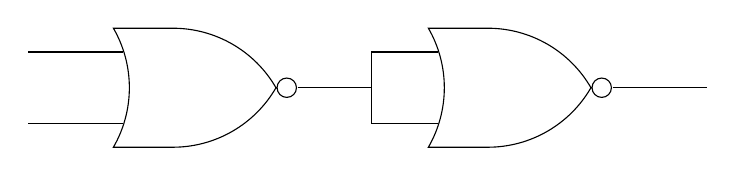
\begin{tikzpicture}[circuit logic US, scale=2]

	\node [nor gate, inputs=nnnn] (gate1) at (0,0) {};
	\node [nor gate, inputs=nnnn] (gate2) at (2,0) {};

	\draw (gate1.output) -- (1.2,0);

	\draw (1.2,0) |- (gate2.input 1);
	\draw (1.2,0) |- (gate2.input 4);

	\draw (gate1.input 1) -- ++(left: 6mm);
	\draw (gate1.input 4) -- ++(left: 6mm);
	\draw (gate2.output) -- ++(right: 6mm);

\end{tikzpicture}
\end{center}

\begin{figure}[H]
\includegraphics[width=7cm]{C39}
\includegraphics[width=7cm]{C40}
\includegraphics[width=7cm]{C41}
\includegraphics[width=7cm]{C42}
\centering
\captionsetup{labelformat=empty}
\caption{}
\end{figure}

\begin{center} 
\textbf{NOT} - negacja \\
\nl
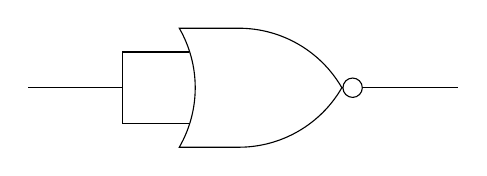
\begin{tikzpicture}[circuit logic US, scale=2]

	\node [nor gate, inputs=nnnn] (gate2) at (2,0) {};

	\draw (1.2,0) -- ++(left: 6mm);

	\draw (1.2,0) |- (gate2.input 1);
	\draw (1.2,0) |- (gate2.input 4);

	\draw (gate2.output) -- ++(right: 6mm);

\end{tikzpicture}
\end{center}

\begin{figure}[H]
\includegraphics[width=7cm]{C43}
\includegraphics[width=7cm]{C44}
\centering
\captionsetup{labelformat=empty}
\caption{}
\end{figure}


\newpage
\paragraph{Ćwiczenie 4.4 \\}
Zmontowanie generatora zbudowanego z trzech bramek NAND. Zmie- rzenie średniego czasu propagacji impulsu przez bramkę mierząc okres drgań generatora. Porównać czasy propagacji bramek NAND na układach scalonych serii podstawowej 7400 i bramek z serii szybkiej 74S00.

\begin{center}
\begin{tikzpicture}[circuit logic US, scale=2]

	\node [nand gate, inputs=nnnn] (nand1) at (0,0) {};
	\node [nand gate, inputs=nnnn] (nand2) at (2,0) {};
	\node [nand gate, inputs=nnnn] (nand3) at (4,0) {};

	\draw (nand1.output) -- (1.2,0);
	\draw (nand2.output) -- (3.2,0);
	\draw (nand3.output) -- (5.2,0);

	\draw (-1.4,0) -- (-0.8,0) |- (nand1.input 1);
	\draw (-0.8,0) |- (nand1.input 4);

	\draw (1.2,0) |- (nand2.input 1);
	\draw (1.2,0) |- (nand2.input 4);

	\draw (3.2,0) |- (nand3.input 1);
	\draw (3.2,0) |- (nand3.input 4);

	\draw (5.2,0) -- (5.2,1) -- (-1.4,1) -- (-1.4,0);
	\draw (5.2,0) -- node[at end, right]{WY} (5.8,0);
	
\end{tikzpicture}
\end{center}

Zmontowałem generator według powyższego schematu na płytce UC-2 i podpiąłem jego wyjście pod oscyloskop. Zmierzyłem okres fal na wyjściu wstawiając w gniazdo na płytce raz układ 7400, a raz 74S00.

\begin{figure}[H]
\includegraphics[width=16cm]{C45} 
\captionsetup{labelformat=empty}
\centering
\caption{}
\end{figure}

\begin{figure}[H]
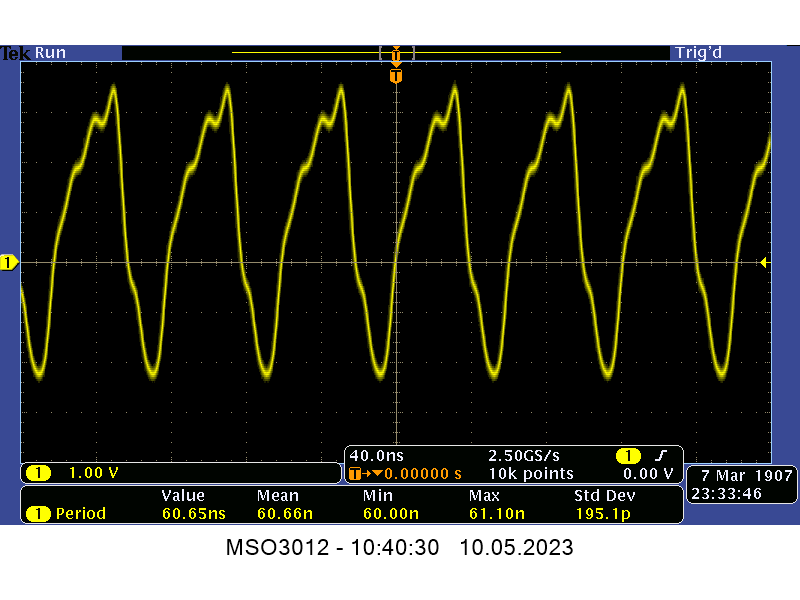
\includegraphics[width=8cm]{A0} 
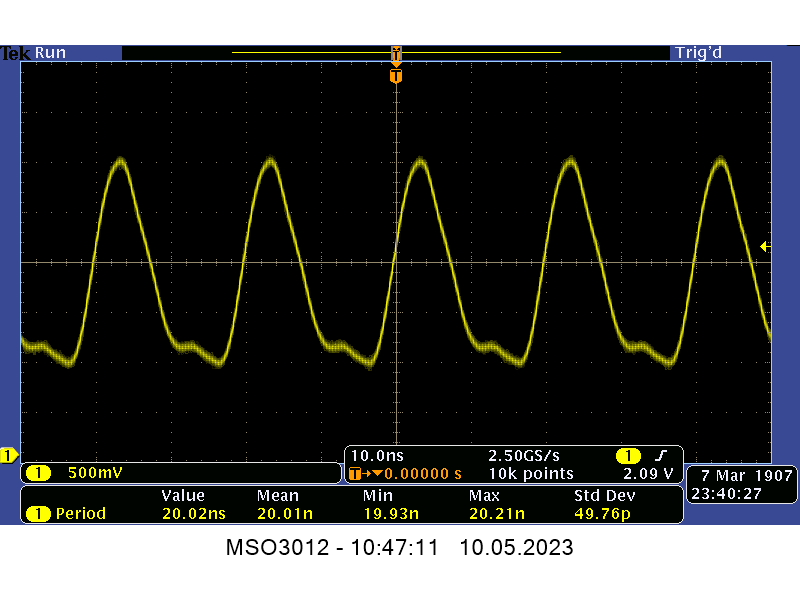
\includegraphics[width=8cm]{A1}
\centering
\captionsetup{labelformat=empty}
\caption{7400 - $60.65 \ ns$ \ \ \ \ \ \ \ \ \ 74S00 - $20.02 \ ns$}
\end{figure}

Zmierzony okres drgań fali powinien być sześciokrotnie większy niż czas propagacji sygnału przez bramkę: $T = 6 \Delta t$. Możemy więc wyliczyć, że średni okres propagacji $t_P$ jest równy: dla układu 7400: $t_P \approx 10.1 \ ns$, dla układu 74S00: $t_P \approx 3.33 \ ns$. \\ 

Jak podaje producent czasy propagacji sygnału bramek serii 7400 powiny spełniać: $t_{PLH} \leq 22 \ ns$ (\textit{propagation low-to-high}) oraz $t_{PHL} \leq 15 \ ns$ (\textit{propagation high-to-low}). Natomiast bramki 74S00: $t_{PLH} \leq 4.5 \ ns$ i $t_{PHL} \leq 5 \ ns$. (Według Texas Instruments Inc. - \textit{SNx400, SNx4LS00, and SNx4S00 Quadruple 2-Input Positive-NAND Gates}, december 1983 – revised may 2017). \\

Zmierzone przeze mnie czasy propagacji są z dużym marginesem w limitach, które gwarantuje producent. Widać także różnice pomiędzy serią podstawową 7400 a serią szybką 74S00, której czas propagacji jest trzykrotnie krótszy.

\newpage
\paragraph{Ćwiczenie 4.5 \\}
Zbudowanie układu realizującego funkcję logiczną dla jednego segmentu wyświetlacza 7-segmentowego, którego zadaniem będzie wyświetlanie liczb w systemie ósemkowym. \\

Wybrałem segment \textit{c}, czyli pionowy, po prawej na dole. W systemie ósemkowym jest osiem cyfr: 0, 1, 2, 3, 4, 5, 6 i 7. Dla każdej z nich oprócz cyfry 2 segment \textit{c} jest zapalony. Przyjmijmy, że liczbę podajemy na wejście logiki wyświetlacza w postaci binarnej, rozpoczynając od najmniej znaczącego bitu. Dla jednocyfrowej liczby ósemkowej funkcja obsługująca segment \textit{c} o trzech wejściach logicznych A, B, C będzie miała postać:

$$ NOT \ ( \ \textit{A} \ ) \ AND \ \textit{B} \ AND \ NOT \ ( \ \textit{C} \ ) $$

Ponieważ segment ten ma być zgaszony tylko jeżeli wejście B ma sygnał TRUE oraz żadne z pozostałych nie mają TRUE. Funkcja ta sprowadza się do postaci:

$$ NOT \ ( \ \textit{B} \ AND \ ( \ NOT \ ( \ \textit{A} \ OR \ \textit{C} \ ) \ ) \ ) $$

$$ \textit{B} \ NAND \ ( \ \textit{A} \ NOR \ \textit{C} \ ) $$

Co można przedstawić za pomocą schematu:

\begin{center}
\begin{tikzpicture}[circuit logic US, scale=2]

	\node [nand gate, inputs=nnnn] (nand1) at (4,0) {};
	\node [nor gate, inputs=nnnn] (nor1) at (0,1) {};

	\draw (nand1.output) -- ++(right: 8mm);
	\draw (nor1.output) -- ++(right: 12mm) |- (nand1.input 1);
	\draw (nand1.input 4) -- node[at end, left]{B} ++(left: 54.5mm);
	\draw (nor1.input 1) -- node[at end, left]{A} ++(left: 15mm);
	\draw (nor1.input 4) -- node[at end, left]{C} ++(left: 15mm);

\end{tikzpicture}
\end{center}

Przy użyciu układów scalonych 7400 i 7402 zmontowałem powyższy układ. Podając na jego wejście liczby od 0 do 7 w postaci binarnej (widoczne na zółtych diodach) obserwowałem czy segment \textit{c} jest zaświecony czy zgaszony (widoczne na próbniku stanów logicznych).

\begin{figure}[H]
\includegraphics[width=7cm]{C52} 
\includegraphics[width=7cm]{C53} 
\includegraphics[width=7cm]{C54} 
\includegraphics[width=7cm]{C55} 
\includegraphics[width=7cm]{C56} 
\includegraphics[width=7cm]{C57} 
\includegraphics[width=7cm]{C58}
\includegraphics[width=7cm]{C59}
\centering
\captionsetup{labelformat=empty}
\caption{}
\end{figure}

Rozszerzenie powyższej logiki na liczby ósemkowe wielocyfrowe jest bardzo proste. Z uwagi na fakt, że jedna cyfra ósemkowa odpowiada trójce bitów binarnych każdą trójkę wejść logicznych należy przetwarzać i wyświetlać osobno jako osobną cyfrę w systemie ósemkowym.


\newpage
\paragraph{Ćwiczenie 4.6 \\}
Zaprojektowanie i zmontowanie przerzutnika asynchronicznego R-S z funktorów NAND i sprawdzenie tablicy przejść. \\

Przerzutnik typu RS to najprostszy rodzaj przerzutnika asynchronicznego. Jest to układ sekwencyjny, którego sygnał na wyjściu zależy zarówno od stanu na wejściu jak i stanu wewnętrznego. Może być stosowany jako układ pamiętający. Jego nazwa pochodzi z angielskiego \textit{Set-Reset} i opisuje obydwa wejścia tego układu: ustawiające i zerujące. \\

Podając sygnał na wejście ustawiające $S$ ustawiamy wyjście $Q$ na TRUE. Podając sygnał na wejście zerujące $R$ zerujemy wyjście $Q$ (ustawiamy na FALSE). Przerzutnik RS ma także komplementarne wyjście $\overline{Q}$, które ma stan zawsze przeciwny niż $Q$. Kiedy na $S$ i $R$ nie ma sygnału przerzutnik utrzymuje swój stan. Podanie sygnału na obydwa wejścia na raz jest niedozwolone (w praktyce powoduje to sygnał TRUE na obydwu wyjściach $Q$ i $\overline{Q}$). 

\begin{center}
\begin{tikzpicture}[circuit logic US, scale=2]

	\node [nand gate, inputs=nnnn] (nand1) at (0, 0) {};
	\node [nand gate, inputs=nnnn] (nand2) at (0, -2) {};

	\draw (nand1.input 1) -- node[at end, left]{$S$} ++(left: 1cm);
	\draw (nand1.input 4) -- ++(left: 5mm) -- ++(down: 5mm) -- (2,-1.7) -- (2,-2);
	\draw (nand1.output) -- ++(right: 4mm) -- (2,0) -- node[at end, right]{$Q$} ++(right: 1cm);

	\draw (nand2.input 4) -- node[at end, left]{$R$} ++(left: 1cm);
	\draw (nand2.input 1) -- ++(left: 5mm) -- ++(up: 5mm) -- (2,-0.3) -- (2,0);
	\draw (nand2.output) -- ++(right: 4mm) -- (2,-2) -- node[at end, right]{$\overline{Q}$} ++(right: 1cm);

\end{tikzpicture}
\end{center}

Warto zaznaczyć, że przerzutnik RS zbudowany na bramkach NAND powinien mieć wejścia normalizowane do sygnału wysokiego (to znaczy, że TRUE i TRUE, w naszym przypadku $5 \ V$, na obydwu wejściach powinno być domyślne) - "Podanie sygnału" oznacza podanie sygnału niskiego ($0 \ V$). Z tego powodu podłączyłem na wejścia zmontowanego przeze mnie przerzutnika wyjścia $\overline{Q}$ impulsatorów - gdy naciskałem przycisk na jedno z wejść przerzutnika trafiał sygnał $0 \ V$ (logiczne FALSE). \\

Tabela stanów przerzutnika RS zbudowanego z bramek NAND:

{
\centering
\begin{center}
\begin{tabular}{ | c | c | c | } 
  \hline
  \ \ \ \textbf{S} \ \ \ & \ \ \ \textbf{R} \ \ \ & \textbf{Q} \\ 
  \hline
  0 & 0 & stan zabroniony \\
  \hline
  0 & 1 & \textit{(set)} 1 \\
  \hline
  1 & 0 & \textit{(reset)} 0 \\
  \hline
  1 & 1 & stan pamiętania \\
  \hline
\end{tabular}
\end{center}
}


\begin{figure}[H]
\includegraphics[width=14cm]{C47}
\centering
\captionsetup{labelformat=empty}
\caption{Przerzutnik RS}
\end{figure}

\begin{figure}[H]
\includegraphics[width=14cm]{C48}
\centering
\captionsetup{labelformat=empty}
\caption{\textit{Set} - sygnał niski na wejściu ustawiającym $S$}
\end{figure}

\begin{figure}[H]
\includegraphics[width=14cm]{C49}
\centering
\captionsetup{labelformat=empty}
\caption{\textit{Reset} - sygnał niski na wejściu zerującym $R$}
\end{figure}

\begin{figure}[H]
\includegraphics[width=8cm]{C50}
\includegraphics[width=8cm]{C51}
\centering
\captionsetup{labelformat=empty}
\caption{Przerzutnik utrzymuje swój stan}
\end{figure}

\newpage
\paragraph{Omówienie wyników i podsumowanie \\}
Podsumowując wyniki z ćwiczeń 4.1 i 4.2 możemy porównywać odczyty oscyloskopu/miernika oraz próbnika stanów logicznych. Możemy zakładać, że "idealnym" sygnałem oznaczającym logiczną jedynkę jest $5.0 \ V$, natomiast "idealnym" logicznym zerem jest $0.0 \ V$. Widzimy jednak, że na wyjściach bramek pojawia się pewna niedokładność: sygnały prawdziwe mają około $4.2 \ V$ a sygnały fałszywe kilkaset miliwoltów. Ta niedokładność z pewnością propaguje się kiedy łączymy bramki w większe układy, wyjście jednej do wejścia drugiej. Próbnij stanów logicznych jednak sobie radzi z rozpoznawaniem poprawnych wartości. \\

O niedokładnościach bramek logicznych oraz o różnicach pomiędzy różnymi seriami (jak mogłoby się wydawać) identycznych bramek uczy także ćwiczenie 4.4. Tranzystory w układach bramek logicznych serii 74, mimo tego, że szybsze i wydajniejsze niż używane dawniej lampy próżniowe, nadal nie są natychmiastowe. Oczywiście, w nowoczesnych procesorach czy układach pamięci, których częstotliwość taktowania to kilka gigaherców używane są znacznie, znacznie szybsze (i droższe) tranzystory półprzewodnikowe. \\

Ćwiczenie 4.3 doskonale pokazuje wszechstronność bramek NAND oraz NOR. Każdą funkcję logiczną da się utworzyć za ich pomocą, co czyni je najczęściej używanymi w nowoczesnych układach. \\

Całe to ćwiczenie jest także dowodem na to, że wynalezienie tranzystorów półprzewodnikowych i rozwój TTL (\textit{transistor-transistor-logic}) było jednym z najważniejszych wydarzeń w historii ludzkości, a na pewno w ostatnim stuleciu.



\newpage
\paragraph{Notatki z zeszytu labolatoryjnego \\}
Poniżej załączone są notatki z zeszytu labolatoryjnego, które prowadziłem podczas zajęć wykonując pomiary.

\begin{figure}[H]
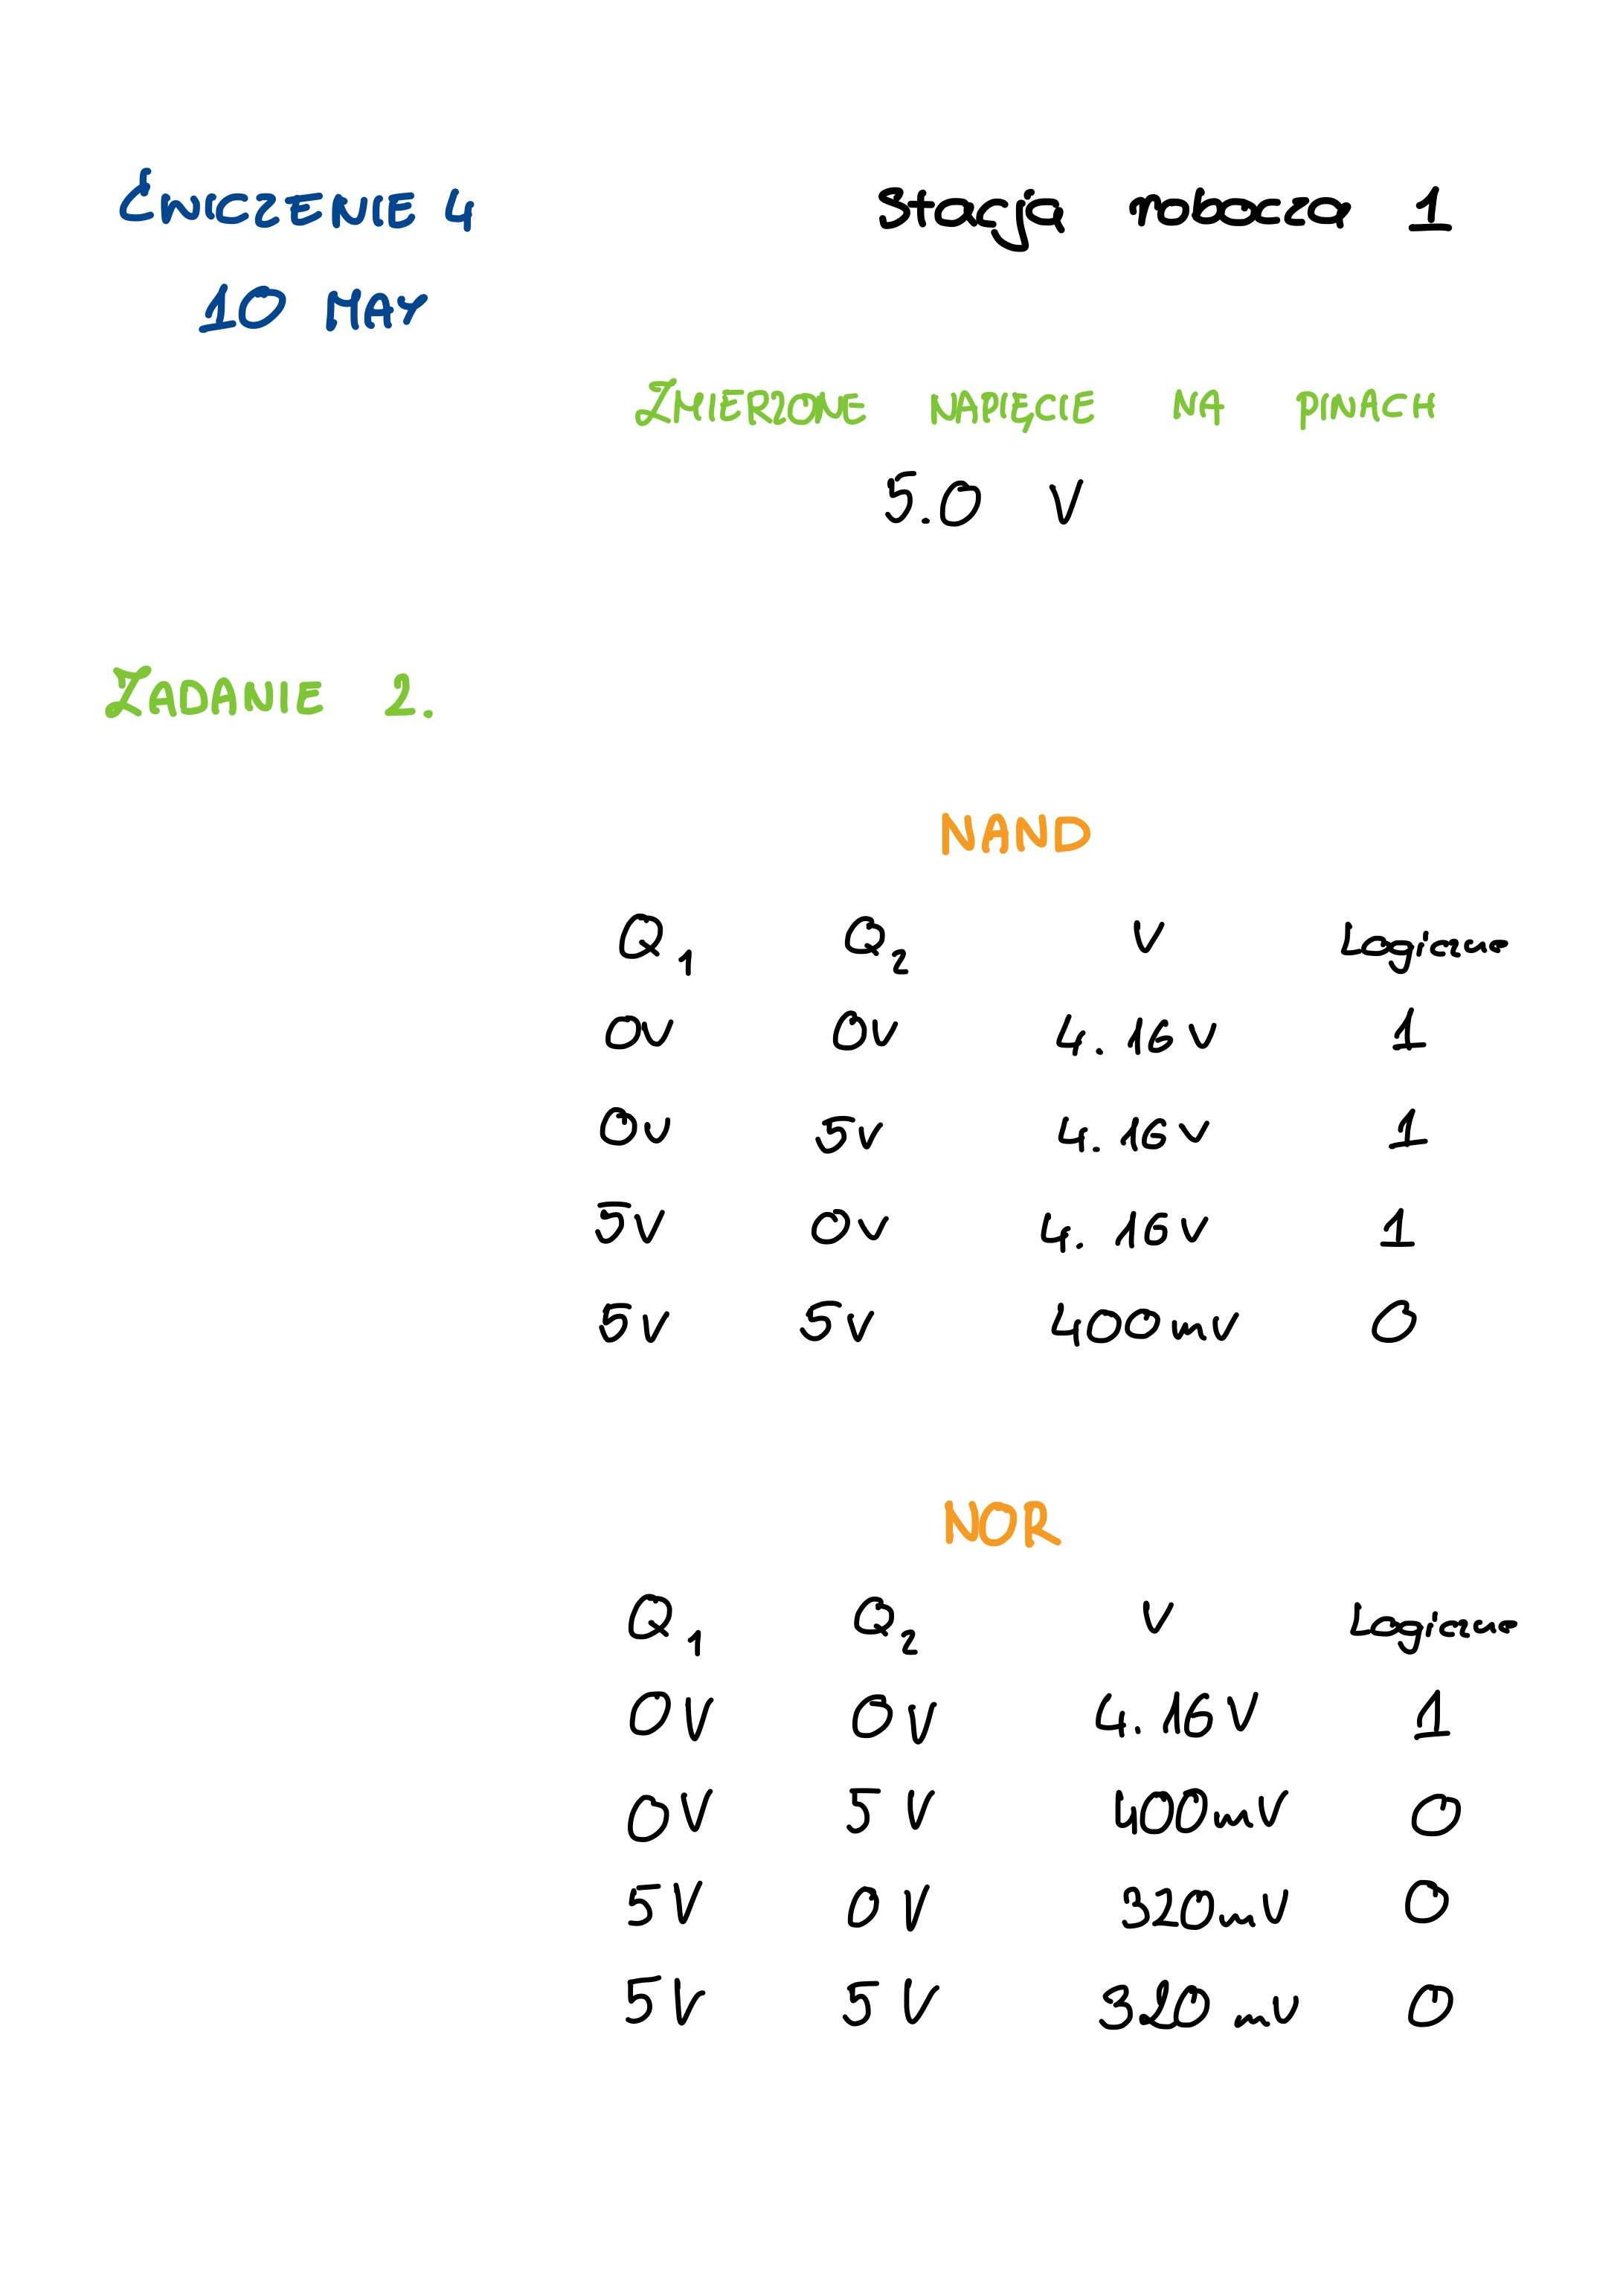
\includegraphics[scale=0.2]{B0}
\centering
\captionsetup{labelformat=empty}
\caption{}
\end{figure}

\begin{figure}[H]
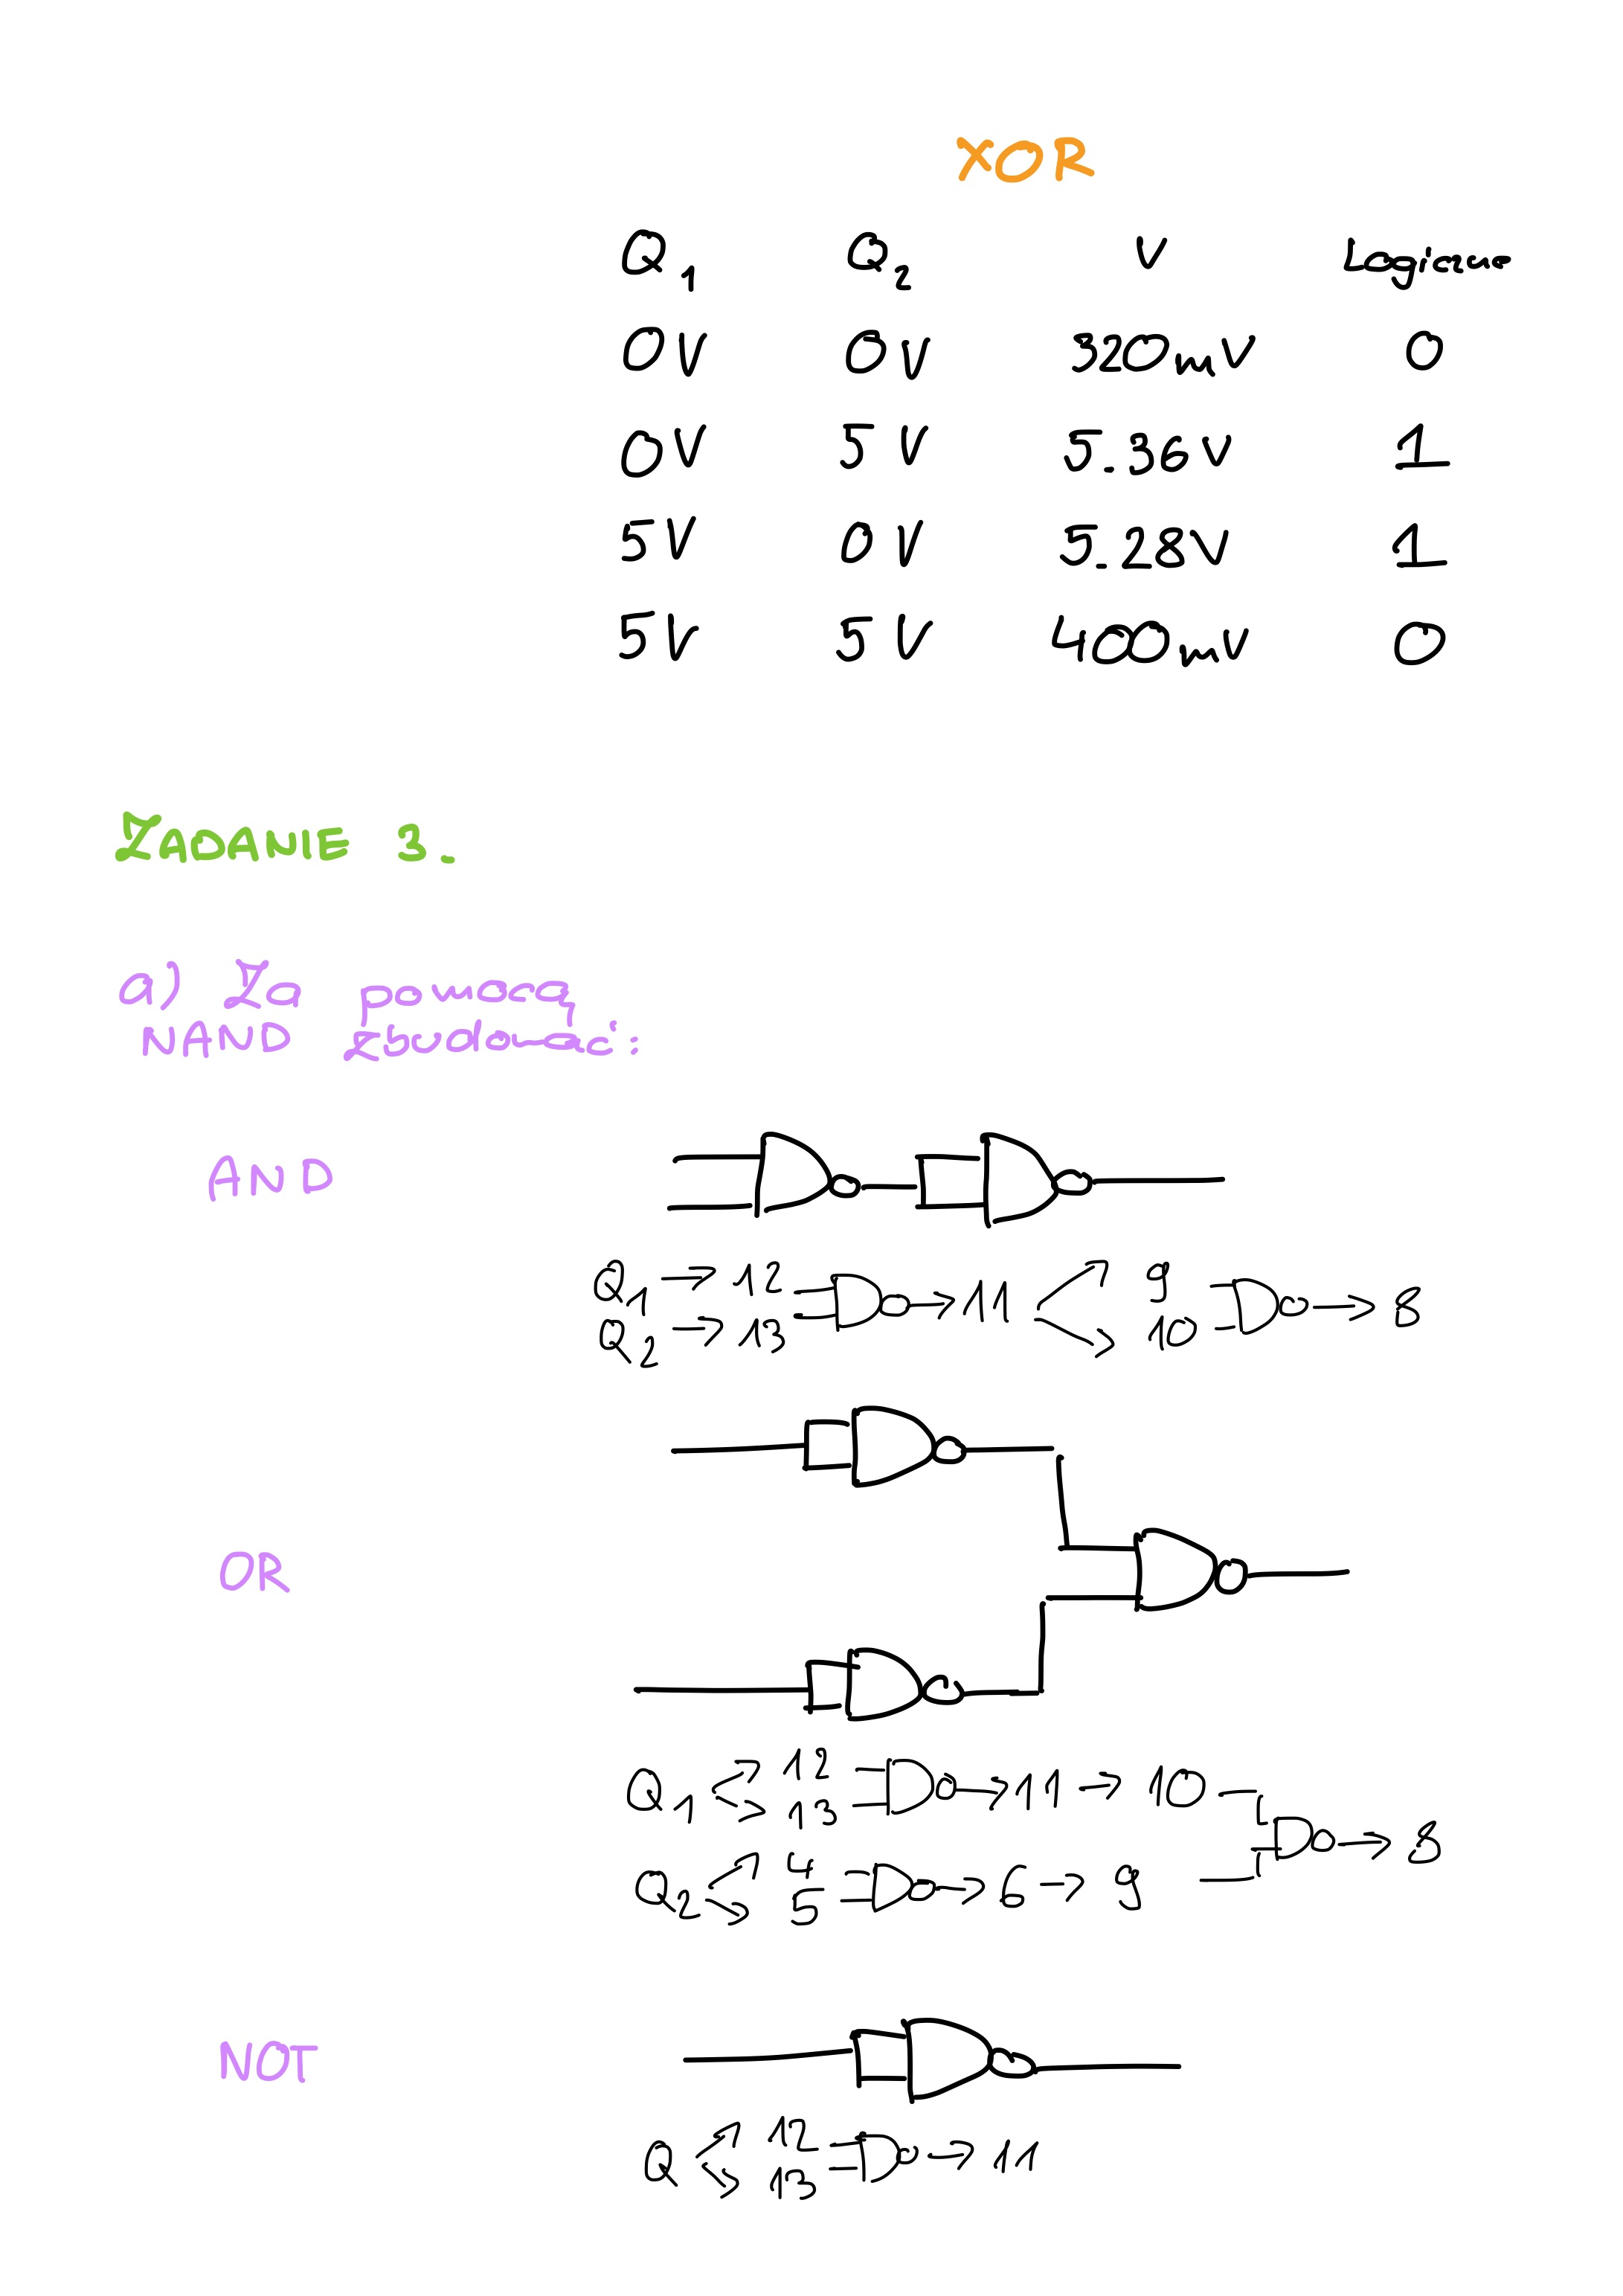
\includegraphics[scale=0.2]{B1}
\centering
\captionsetup{labelformat=empty}
\caption{}
\end{figure}

\begin{figure}[H]
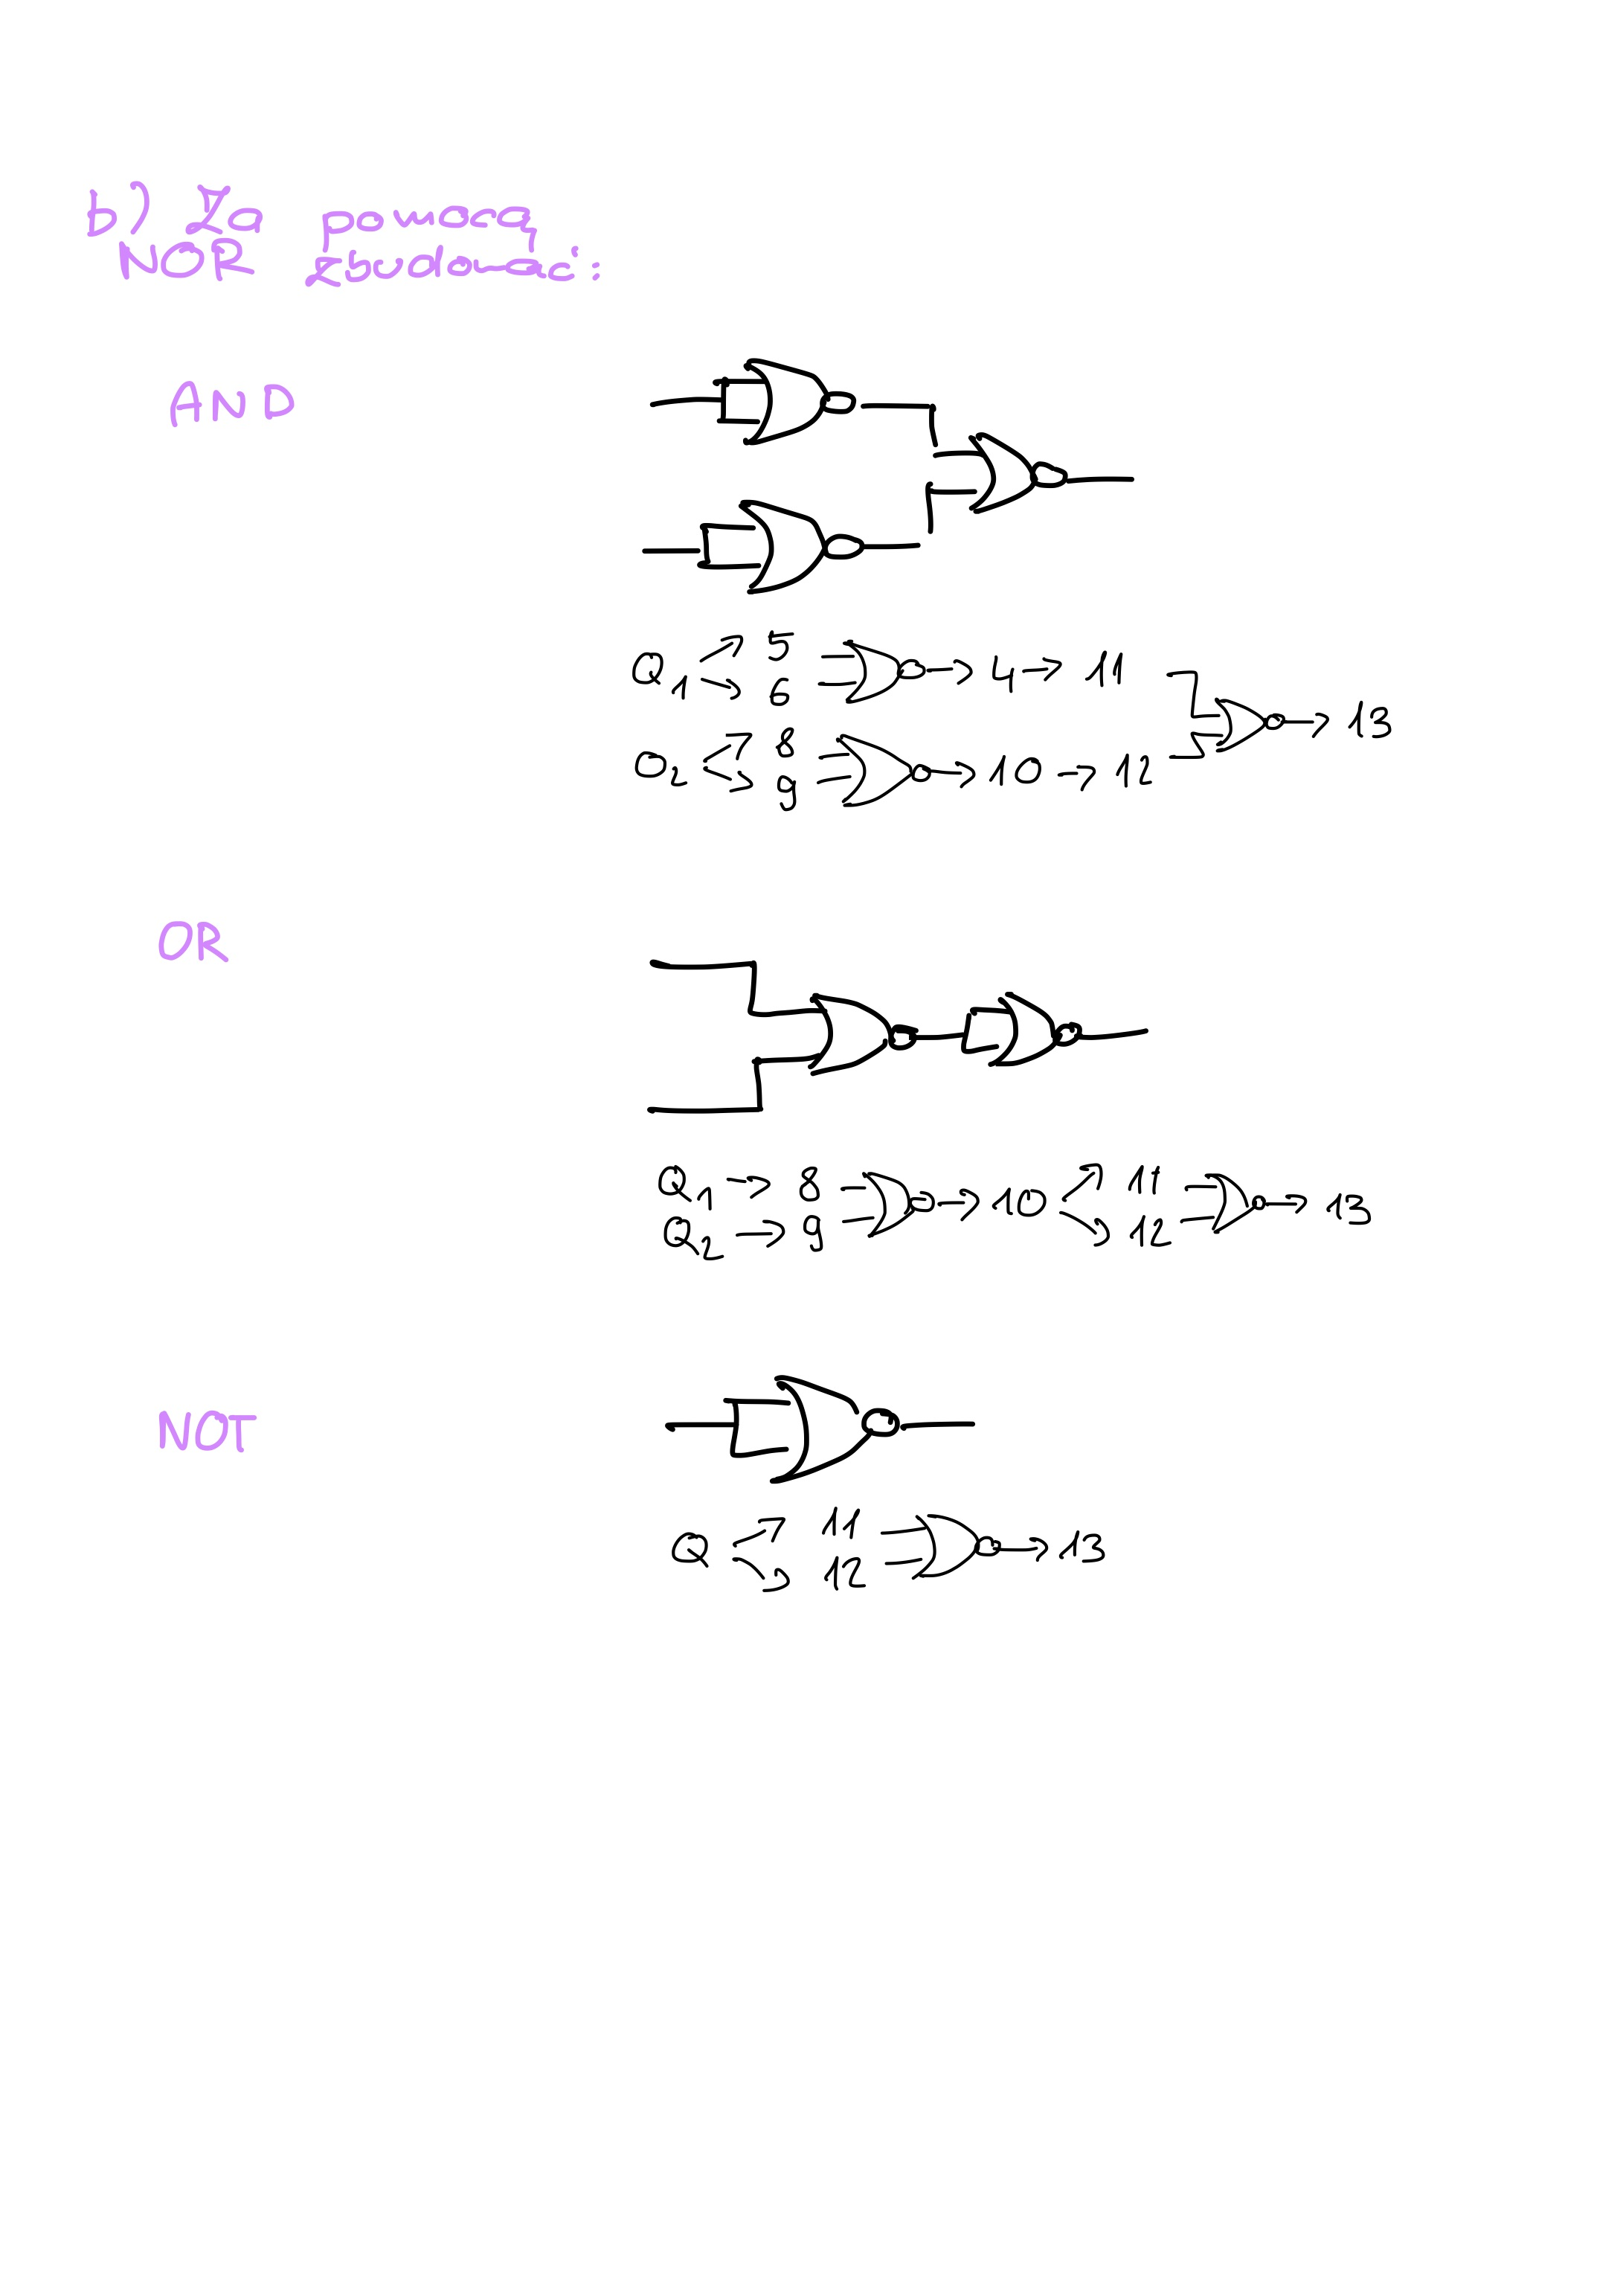
\includegraphics[scale=0.2]{B2}
\centering
\captionsetup{labelformat=empty}
\caption{}
\end{figure}

\begin{figure}[H]
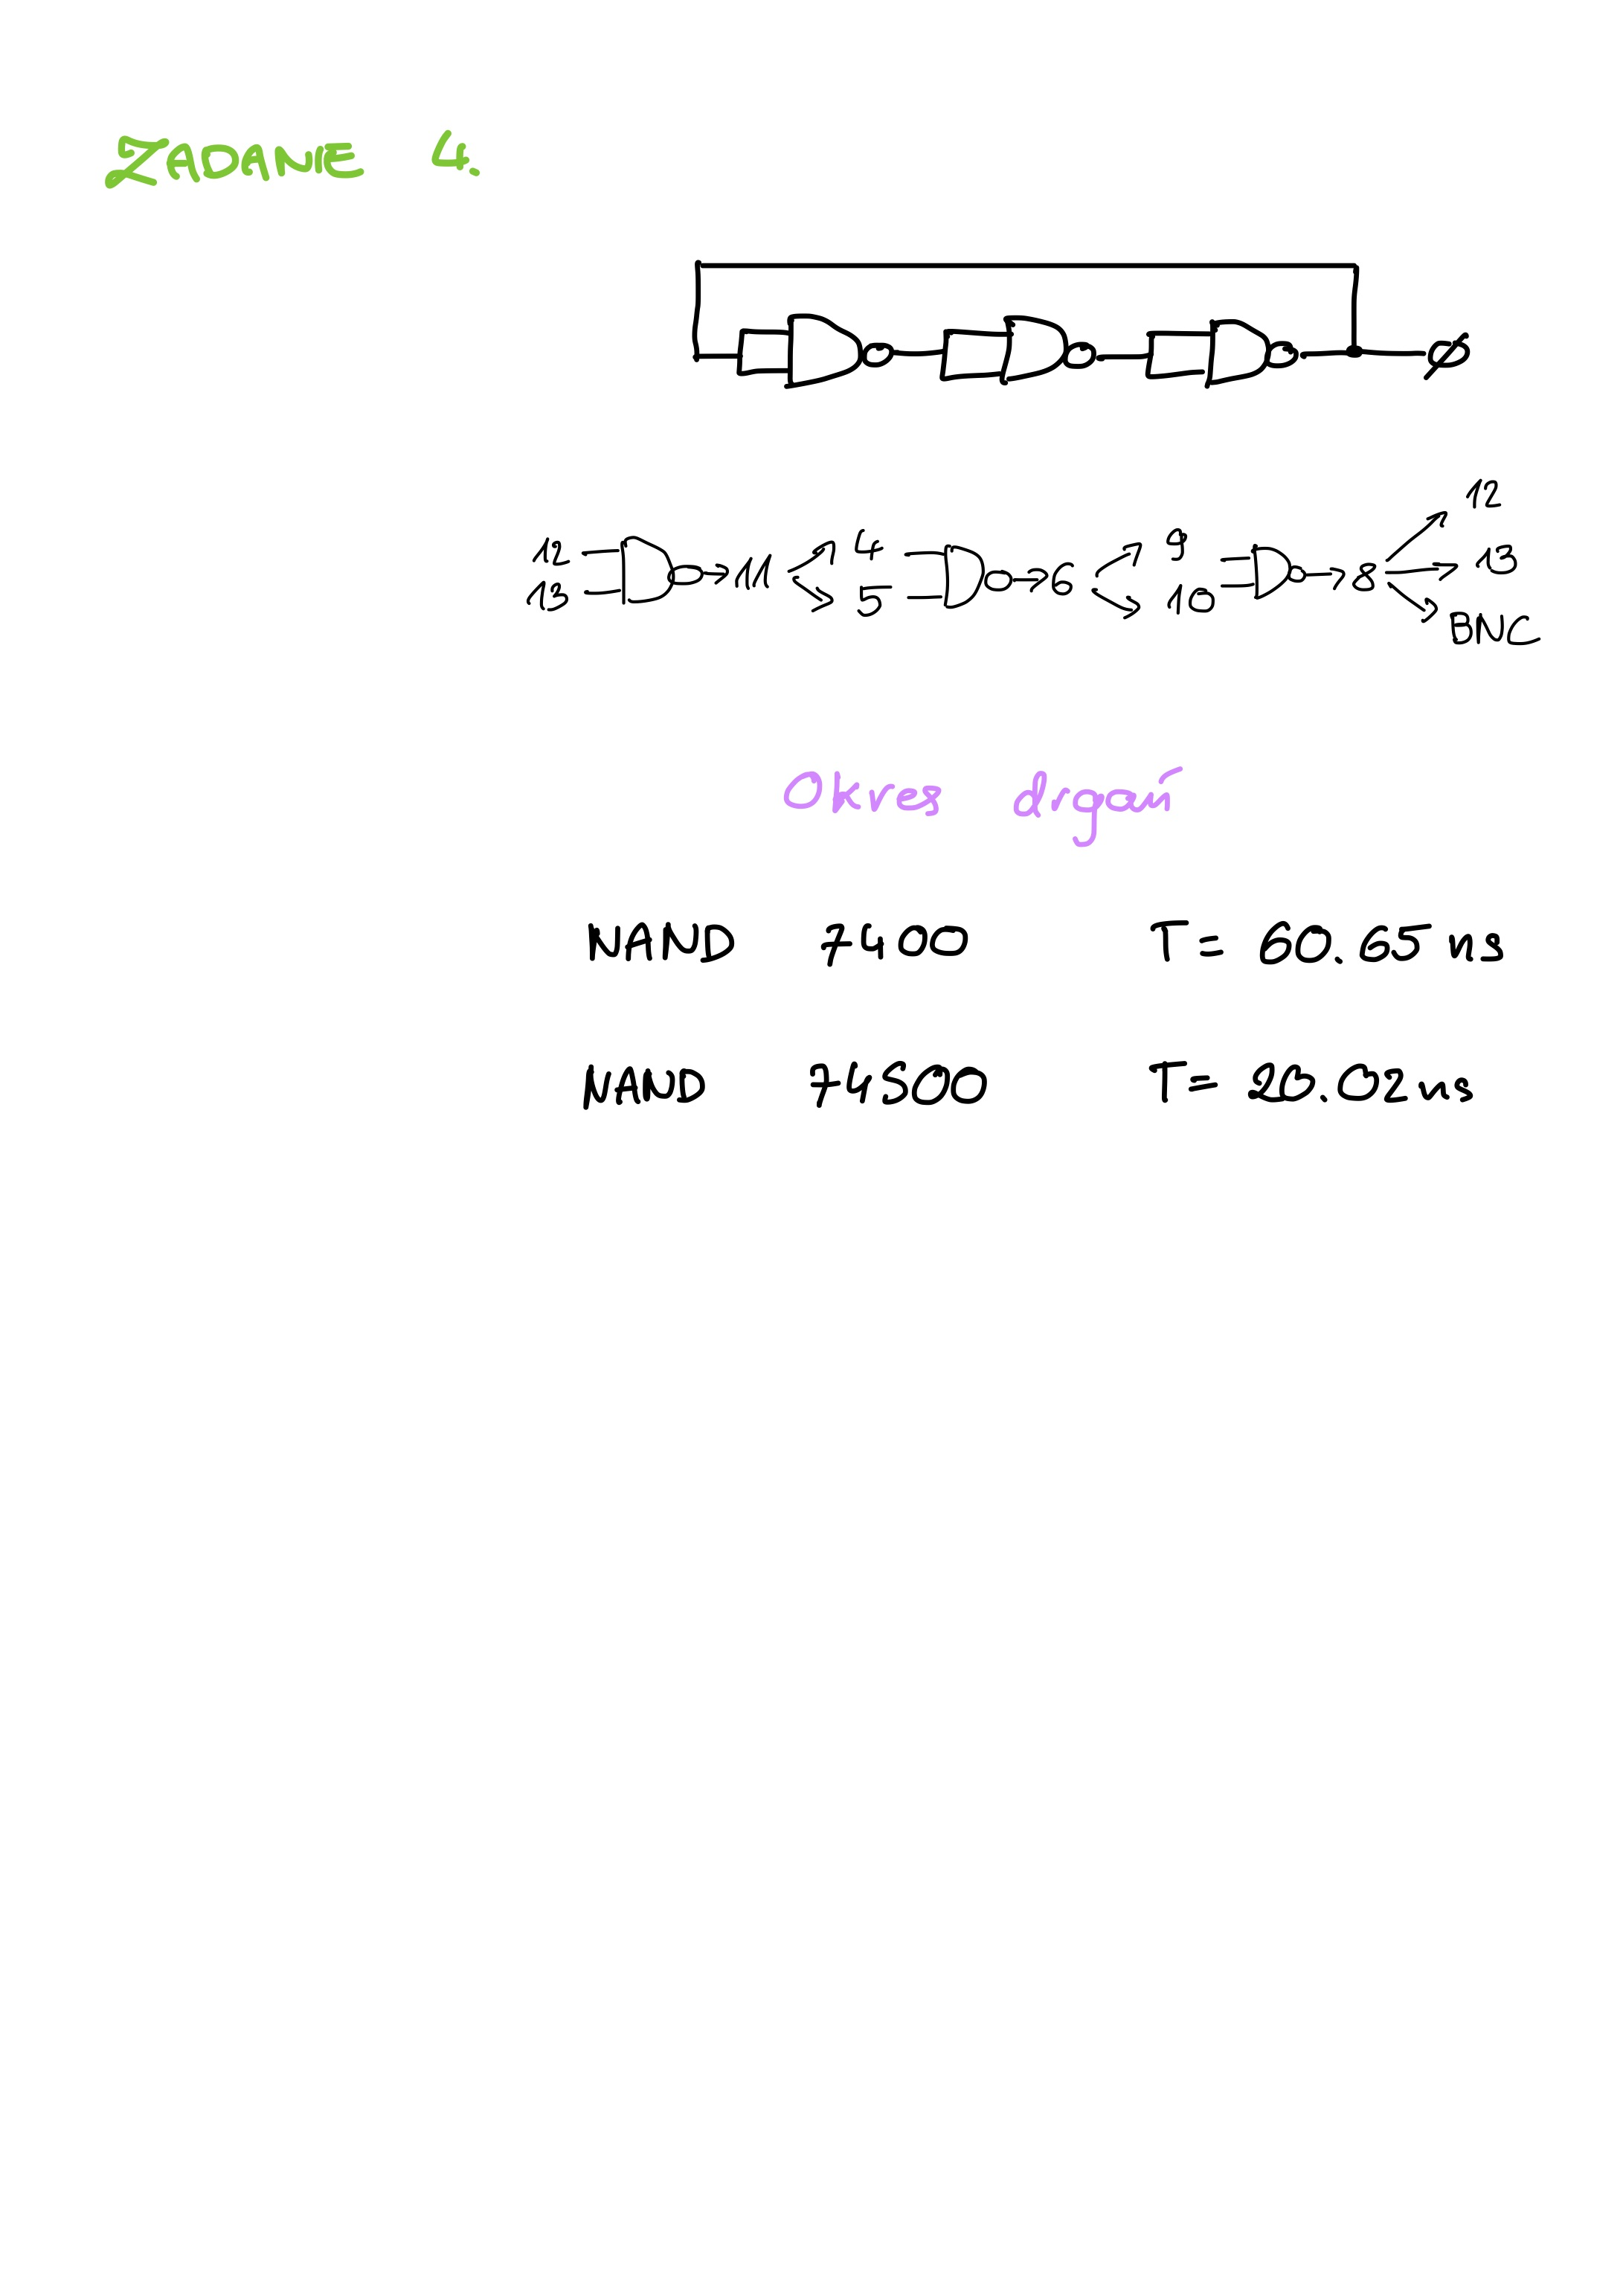
\includegraphics[scale=0.2]{B3}
\centering
\captionsetup{labelformat=empty}
\caption{}
\end{figure}

\begin{figure}[H]
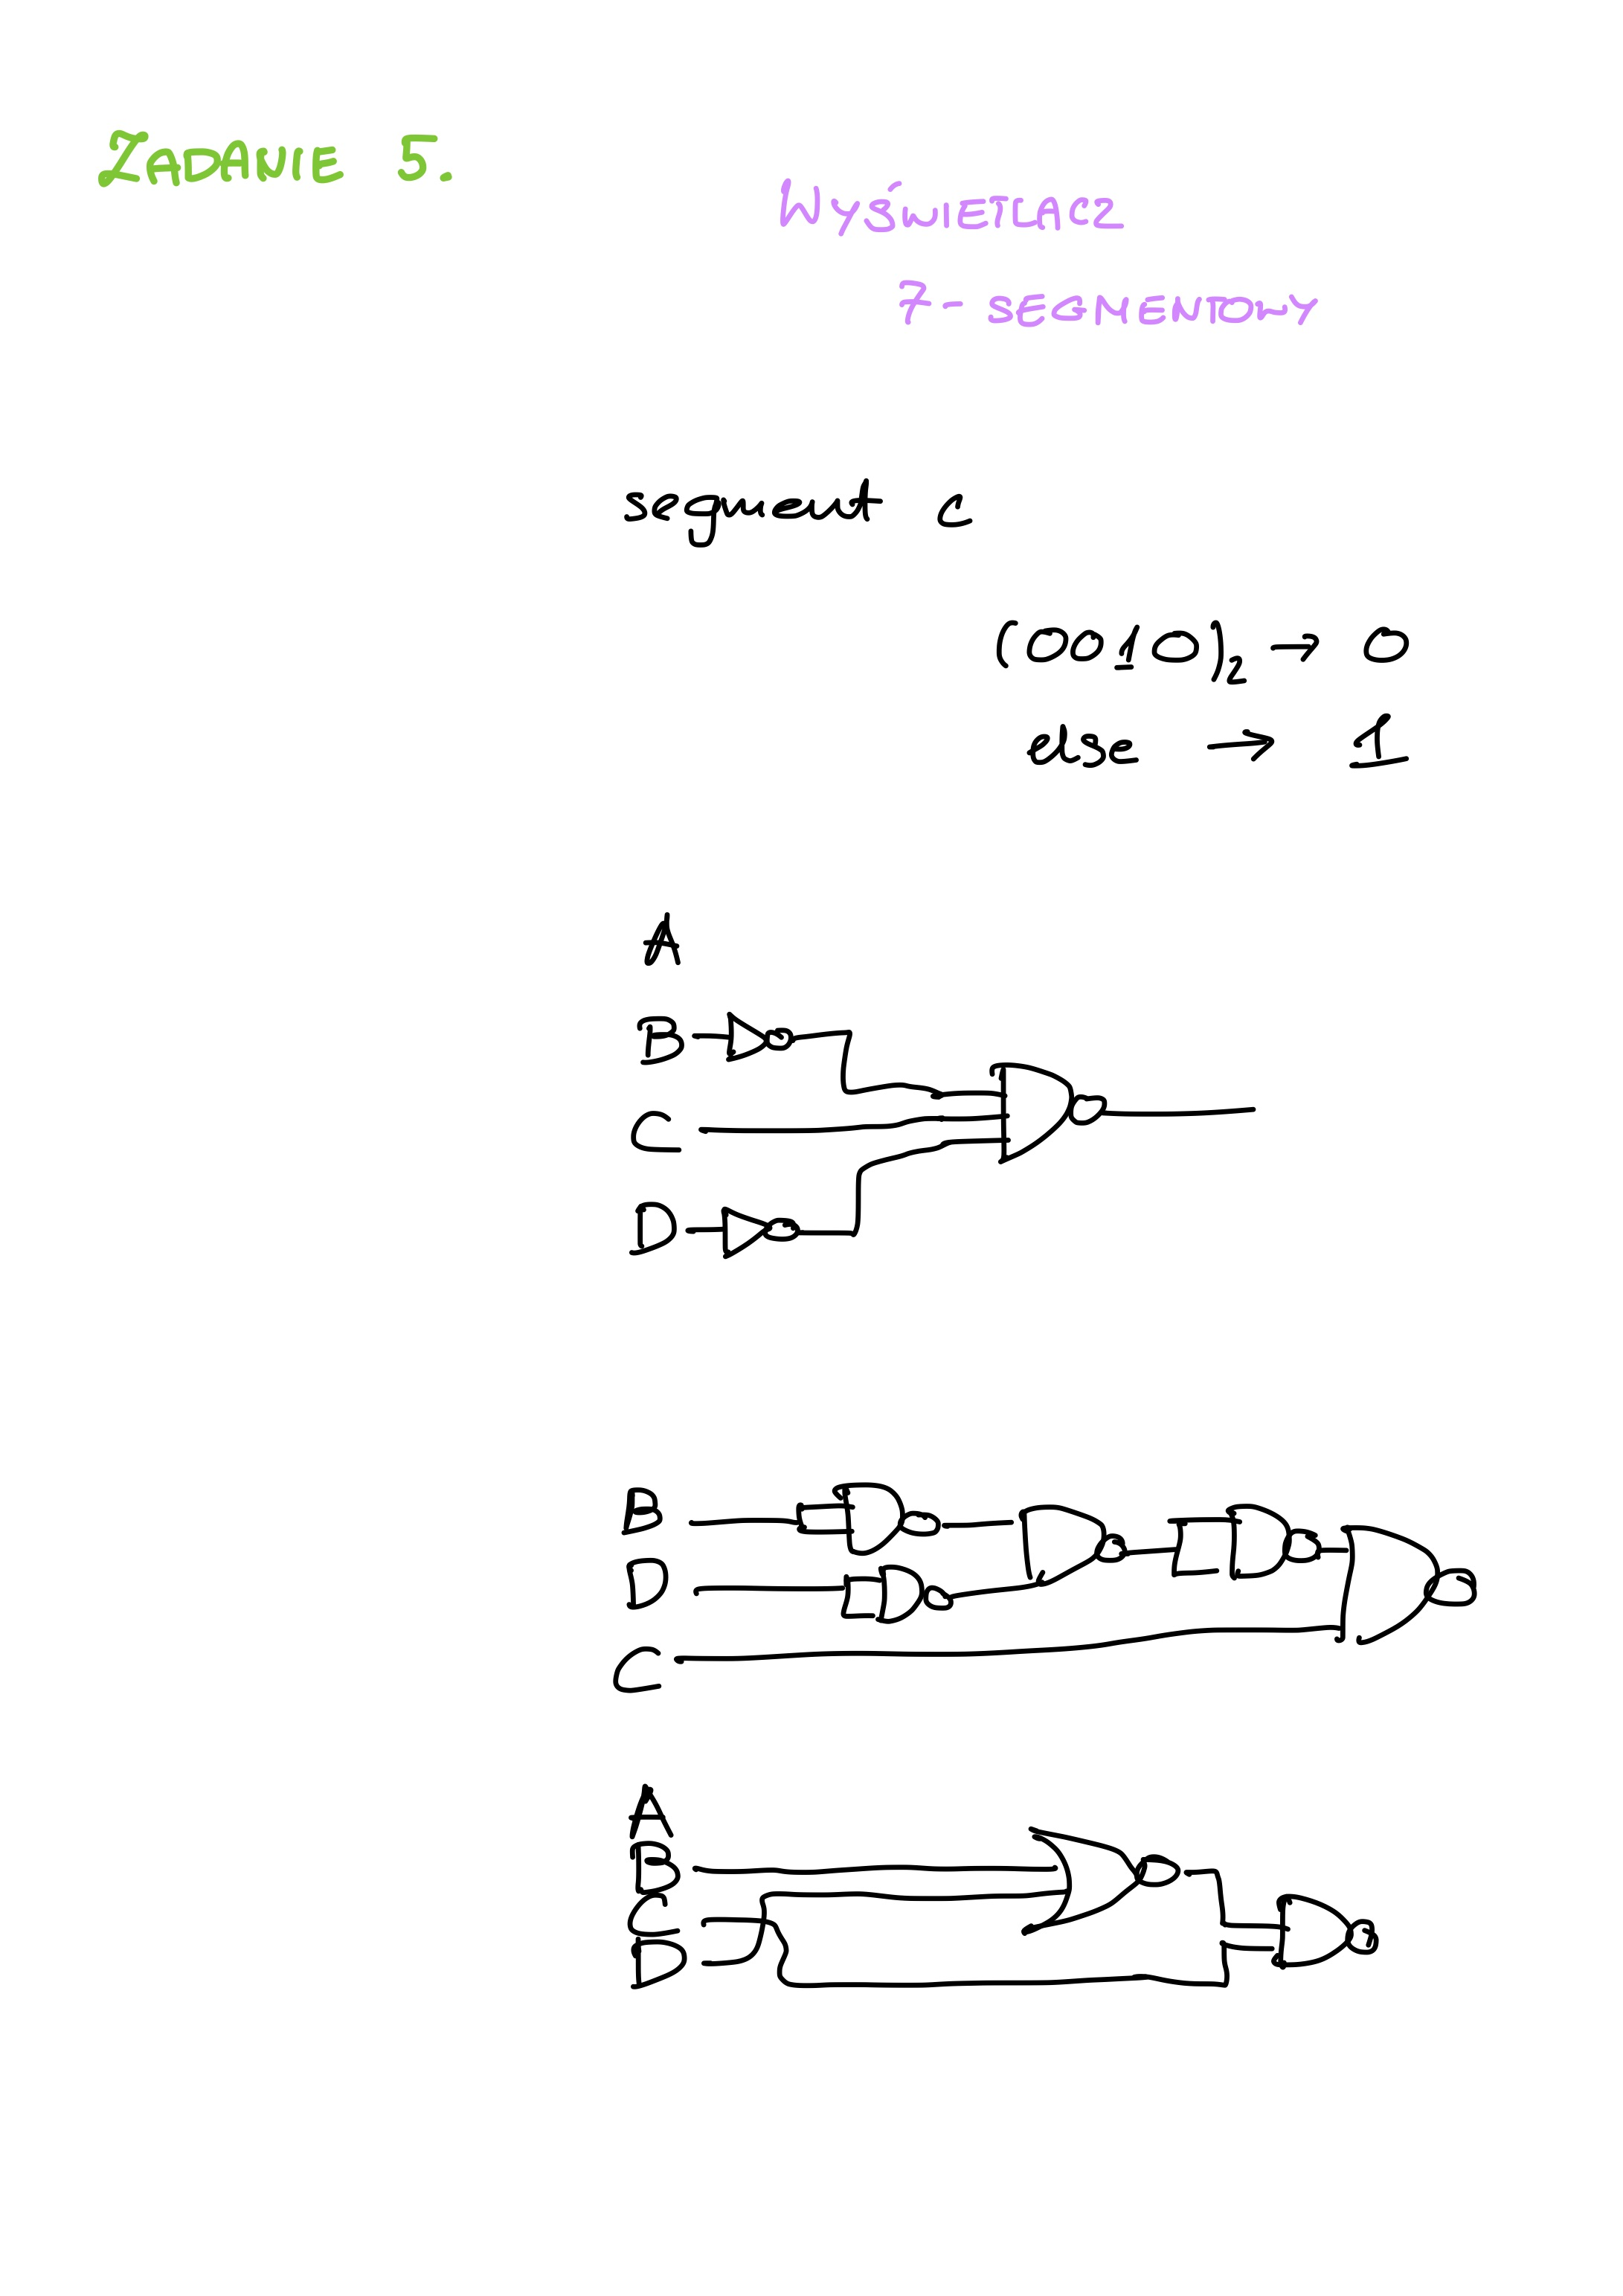
\includegraphics[scale=0.2]{B5}
\centering
\captionsetup{labelformat=empty}
\caption{}
\end{figure}

\begin{figure}[H]
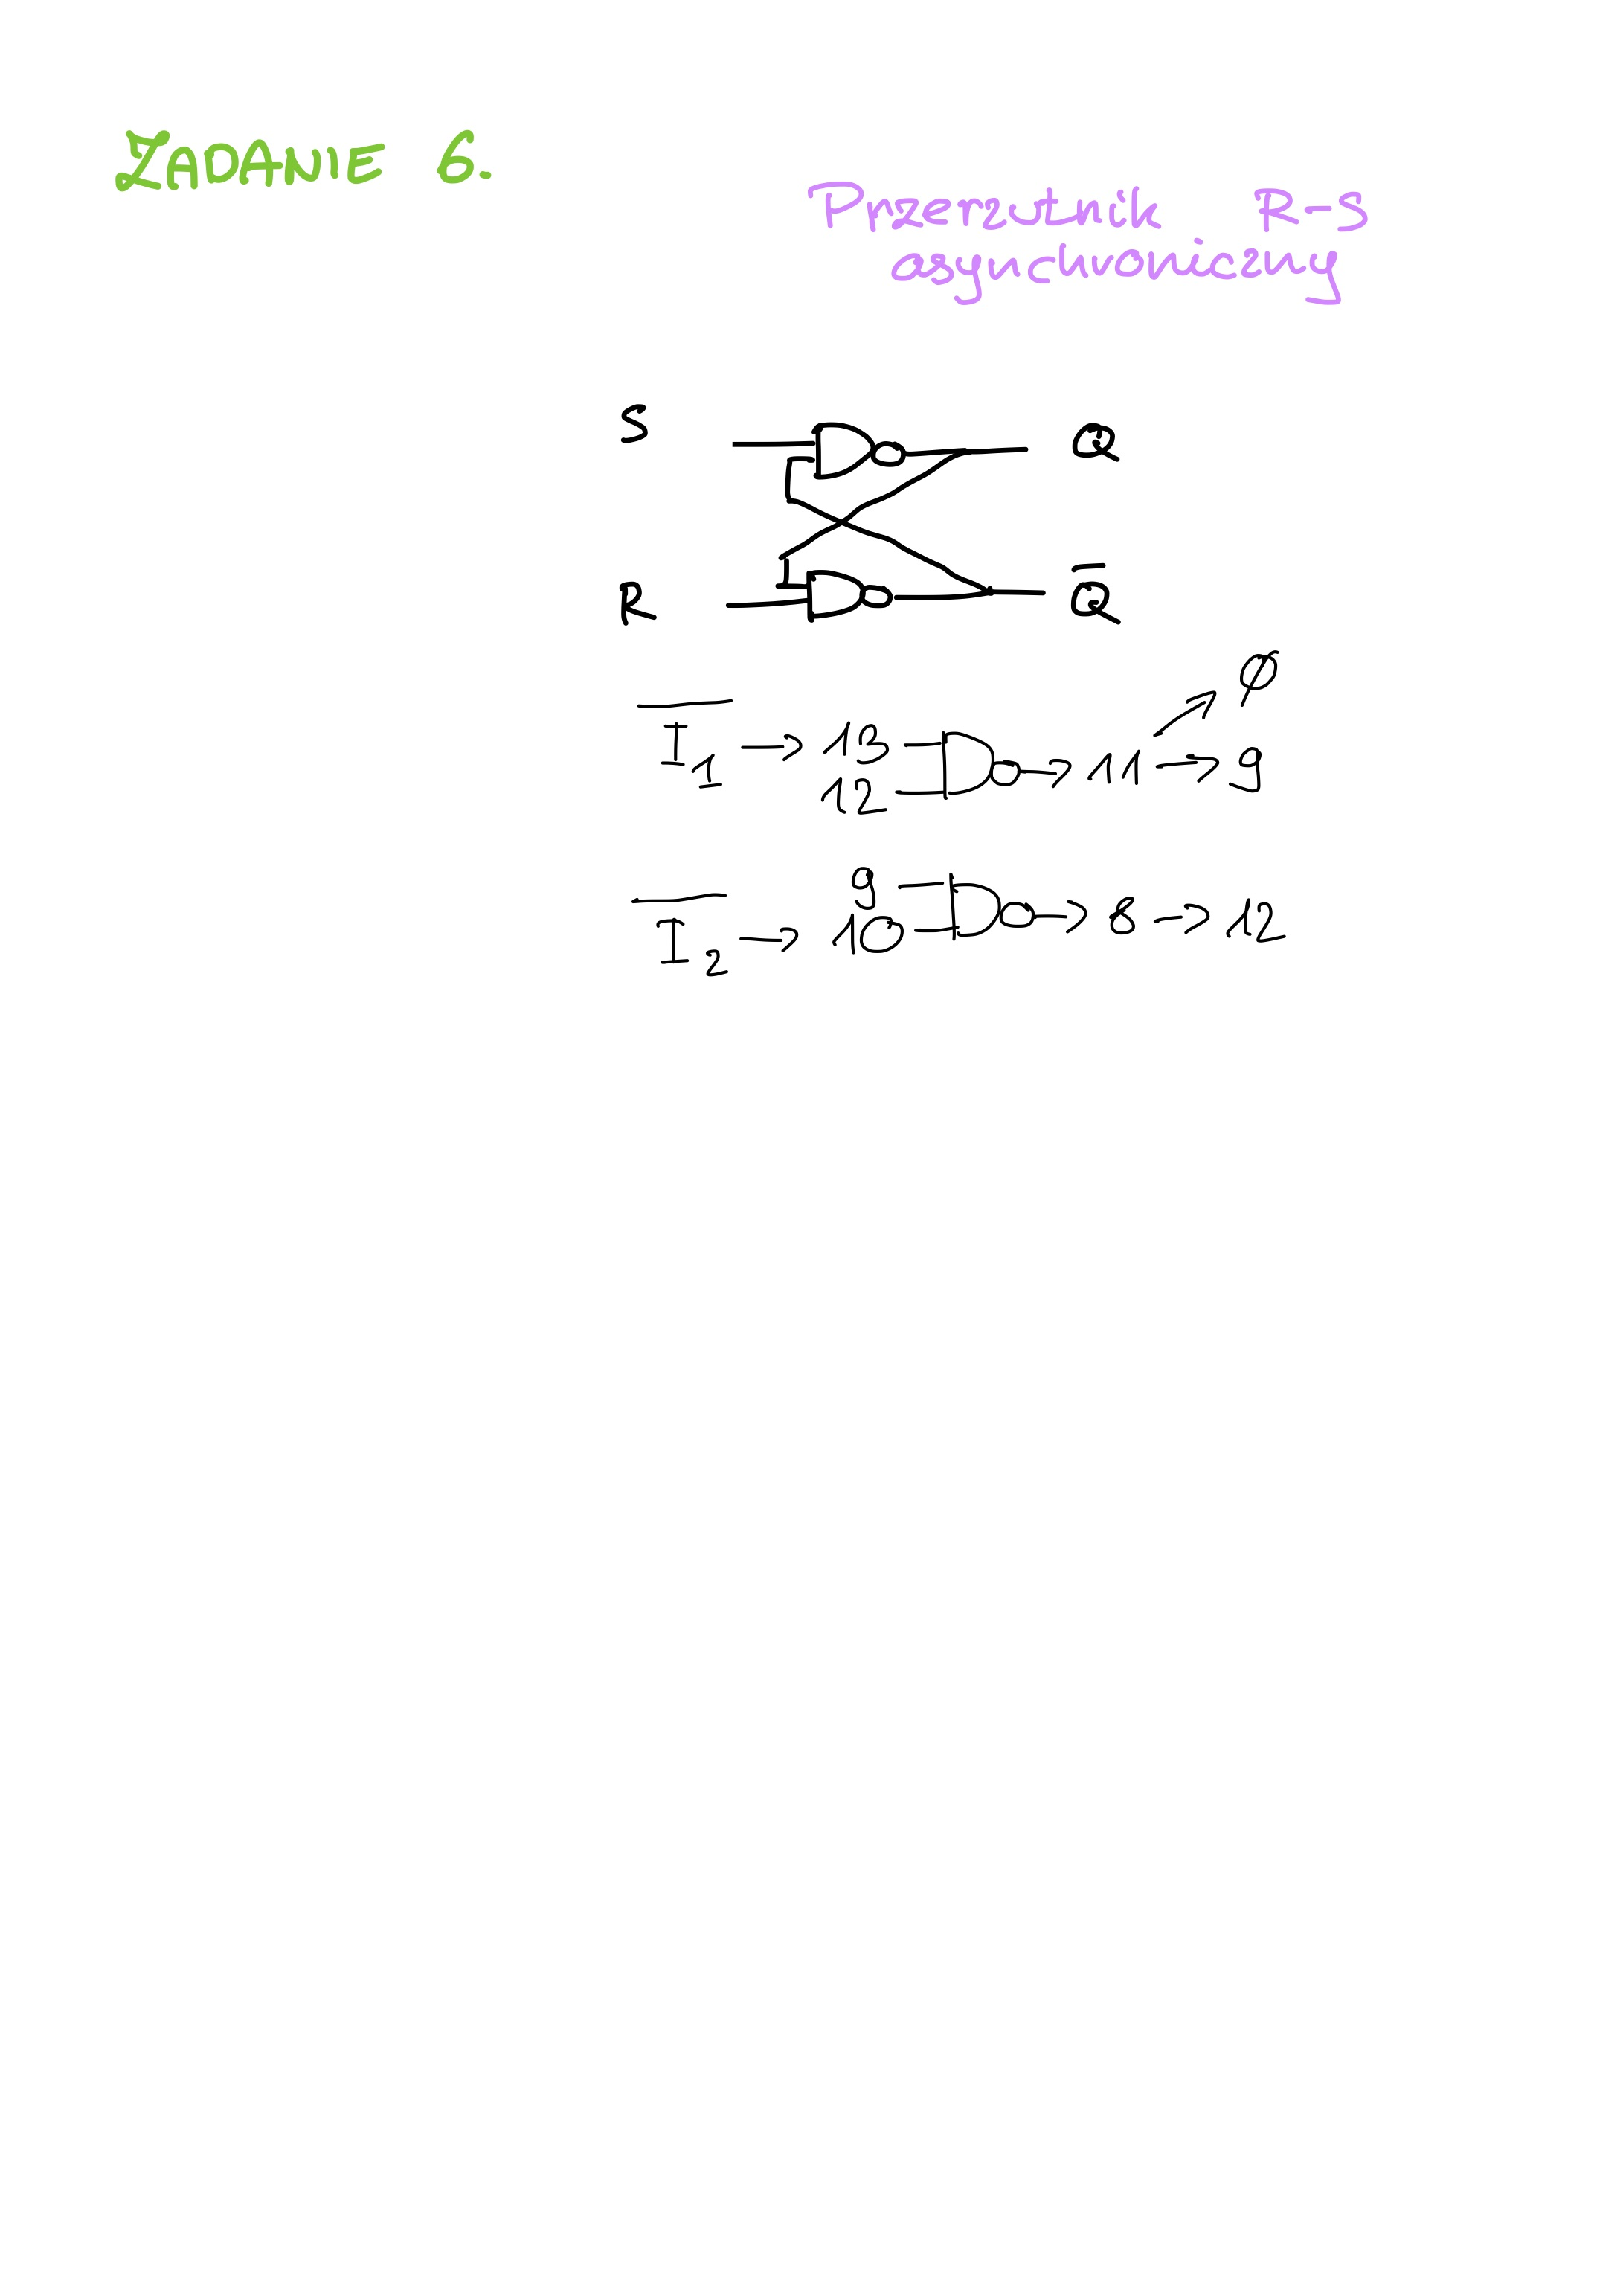
\includegraphics[scale=0.2]{B4}
\centering
\captionsetup{labelformat=empty}
\caption{}
\end{figure}

\end{document}